\documentclass[12pt,a4paper]{report}
%% Verze pro jednostranný tisk:
% Okraje: levý 40mm, pravý 25mm, horní a dolní 25mm
% (ale pozor, LaTeX si sám přidává 1in)
\setlength\textwidth{145mm}
\setlength\textheight{247mm}
\setlength\oddsidemargin{15mm}
\setlength\evensidemargin{15mm}
\setlength\topmargin{0mm}
\setlength\headsep{0mm}
\setlength\headheight{0mm}
% \openright zařídí, aby následující text začínal na pravé straně knihy
\let\openright=\clearpage

% Use additional margin space instead of indented first line to mark new paragraph.
% http://en.wikibooks.org/wiki/LaTeX/Paragraph_Formatting
\usepackage{parskip}

% Allow for more padding in tables.
% http://tex.stackexchange.com/questions/31672/column-padding-in-tables
\usepackage{booktabs}

%% Pokud tiskneme oboustranně:
% \documentclass[12pt,a4paper,twoside,openright]{report}
% \setlength\textwidth{145mm}
% \setlength\textheight{247mm}
% \setlength\oddsidemargin{15mm}
% \setlength\evensidemargin{0mm}
% \setlength\topmargin{0mm}
% \setlength\headsep{0mm}
% \setlength\headheight{0mm}
% \let\openright=\cleardoublepage

% Why use T1 for fontenc package:
% http://tex.stackexchange.com/questions/664/
\usepackage[T1]{fontenc}
% Nice intro to LaTeX fonts: http://www-h.eng.cam.ac.uk/help/tpl/textprocessing/fonts.html
% Better list of font families: http://www.macfreek.nl/memory/Fonts_in_LaTeX#Specifying_Fonts_to_Use
\usepackage{lmodern} % to set monospace to LM Typewriter
\usepackage{mathpazo} % to set roman to Palatino

%% Použité kódování znaků: obvykle latin2, cp1250 nebo utf8:
\usepackage[utf8]{inputenc}

%% Balíčky doporučené skrz http://repo.or.cz/w/csplainnat.git
\usepackage[round]{natbib}      % sazba pouzite literatury
\usepackage{url}                % sazba URL

%% Ostatní balíčky
\usepackage{graphicx}
\usepackage{amsmath}
\usepackage{amsthm}
\usepackage{amssymb}

% Allows for nice typesetting of quotes at the beginning of chapters
% (not sure, if this is allowed in master thesis, but what the hell):
% http://tex.stackexchange.com/questions/53377/
\usepackage{epigraph}

% Allows for continuous footnotes numbering:
% http://tex.stackexchange.com/questions/10448/
\usepackage{chngcntr}
\counterwithout{footnote}{chapter}

% Redefines the underscore symbol so that you don't have to escape it in text mode:
% http://stackoverflow.com/a/1346534
\usepackage{underscore}

%% Balíček hyperref, kterým jdou vyrábět klikací odkazy v PDF,
%% ale hlavně ho používáme k uložení metadat do PDF (včetně obsahu).
%% POZOR, nezapomeňte vyplnit jméno práce a autora.
\usepackage[ps2pdf,unicode]{hyperref}   % Musí být za všemi ostatními balíčky
\hypersetup{pdftitle=Streamed Phrase Table Extraction}
\hypersetup{pdfauthor=Česlav Przywara}
\hypersetup{colorlinks=true} % Better option for PDF file.
%\hypersetup{colorlinks=false} % Better option for print.

%%% Drobné úpravy stylu

% Tato makra přesvědčují mírně ošklivým trikem LaTeX, aby hlavičky kapitol
% sázel příčetněji a nevynechával nad nimi spoustu místa. Směle ignorujte.
\makeatletter
\def\@makechapterhead#1{
  {\parindent \z@ \raggedright \normalfont
   \Huge\bfseries \thechapter. #1
   \par\nobreak
   \vskip 20\p@
}}
\def\@makeschapterhead#1{
  {\parindent \z@ \raggedright \normalfont
   \Huge\bfseries #1
   \par\nobreak
   \vskip 20\p@
}}
\makeatother

% Toto makro definuje kapitolu, která není očíslovaná, ale je uvedena v obsahu.
\def\chapwithtoc#1{
\chapter*{#1}
\addcontentsline{toc}{chapter}{#1}
}

\newtheorem*{definition}{Definition}

% Ondřej's (and my own) definitions
\def\url#1{{\tt{}#1}}
\def\footurl#1{{\footnote{\tt{}#1}}}

\def\Aref#1{Appendix~\ref{#1}}
\def\Cref#1{Chapter~\ref{#1}}
\def\Eref#1{Equation~\ref{#1}}
\def\Fref#1{Figure~\ref{#1}}
\def\Sref#1{Section~\ref{#1}}
\def\Tref#1{Table~\ref{#1}}

\def\Eppex{{\emph{Eppex}}}
\def\eppex{{\emph{eppex}}}


%%%%%%%%%%%%%%%%%%%%%%%%%%%%%%%%%%%%%%%%%%%%%%%%%%%%%%%%%%%%%%%%%%%%%%%%%%%%%%
%%%%%%%%%%%%%%%%%%%%%%%%%%%%%%%%%% DOCUMENT %%%%%%%%%%%%%%%%%%%%%%%%%%%%%%%%%%
%%%%%%%%%%%%%%%%%%%%%%%%%%%%%%%%%%%%%%%%%%%%%%%%%%%%%%%%%%%%%%%%%%%%%%%%%%%%%%

\begin{document}

% Trochu volnější nastavení dělení slov, než je default.
\lefthyphenmin=2
\righthyphenmin=2

%%% Titulní strana práce

\pagestyle{empty}
\begin{center}

\large

Charles University in Prague

\medskip

Faculty of Mathematics and Physics

\vfill

{\bf\Large MASTER THESIS}

\vfill

\centerline{\mbox{
\includegraphics[width=60mm]{logo.eps}}}

\vfill
\vspace{5mm}

{\LARGE Česlav Przywara}

\vspace{15mm}

% Název práce přesně podle zadání
{\LARGE\bfseries Streamed Phrase Table Extraction}

\vfill

% Název katedry nebo ústavu, kde byla práce oficiálně zadána (dle Organizační struktury MFF UK)
Institute of Formal and Applied Linguistics

\vfill

\begin{tabular}{rl}

% TODO: Tesne pred tiskem overit, zda Bojar nema nejaky novy titul :)
Supervisor of the master thesis: & RNDr. Ondřej Bojar Ph.D. \\
\noalign{\vspace{2mm}}
Study programme: & Computer Science \\
\noalign{\vspace{2mm}}
Specialization: & Mathematical Linguistics \\
\end{tabular}

\vfill

% Zde doplňte rok
Prague 2013

\end{center}

\newpage

%%% Následuje vevázaný list -- kopie podepsaného "Zadání diplomové práce".
%%% Toto zadání NENÍ součástí elektronické verze práce, nescanovat.

%%% Na tomto místě mohou být napsána případná poděkování (vedoucímu práce,
%%% konzultantovi, tomu, kdo zapůjčil software, literaturu apod.)

\openright

\noindent
%TODO: Thank someone :)

\newpage

%%% Strana s čestným prohlášením k diplomové práci

\vglue 0pt plus 1fill

\noindent
I declare that I carried out this master thesis independently, and only with the cited
sources, literature and other professional sources.

\medskip\noindent
I understand that my work relates to the rights and obligations under the Act No.
121/2000 Coll., the Copyright Act, as amended, in particular the fact that the Charles
University in Prague has the right to conclude a license agreement on the use of this
work as a school work pursuant to Section 60 paragraph 1 of the Copyright Act.

\vspace{10mm}

\hbox{\hbox to 0.5\hsize{%
In .......... date ...............
\hss}\hbox to 0.5\hsize{%
Signature
\hss}}

\vspace{20mm}
\newpage

%%% Povinná informační strana diplomové práce

\vbox to 0.5\vsize{
\setlength\parindent{0mm}
\setlength\parskip{5mm}

Název práce:
Přibližná extrakce frázové tabulky z velkého paralelního korpusu
% přesně dle zadání

Autor:
Česlav Przywara

Katedra:  % Případně Ústav:
Ústav formální a aplikované lingvistiky
% dle Organizační struktury MFF UK

Vedoucí diplomové práce:
RNDr. Ondřej Bojar Ph.D., Ústav formální a aplikované lingvistiky
% dle Organizační struktury MFF UK, případně plný název pracoviště mimo MFF UK

Abstrakt:
% abstrakt v rozsahu 80-200 slov; nejedná se však o opis zadání diplomové práce - TODO

Klíčová slova:
% 3 až 5 klíčových slov - TODO

\vss}\nobreak\vbox to 0.49\vsize{
\setlength\parindent{0mm}
\setlength\parskip{5mm}

Title:
Streamed Phrase Table Extraction
% přesný překlad názvu práce v angličtině

Author:
Česlav Przywara

Department:
Institute of Formal and Applied Linguistics
% dle Organizační struktury MFF UK v angličtině

Supervisor:
RNDr. Ondřej Bojar Ph.D., Institute of Formal and Applied Linguistics
% dle Organizační struktury MFF UK, případně plný název pracoviště
% mimo MFF UK v angličtině

Abstract:
% abstrakt v rozsahu 80-200 slov v angličtině; nejedná se však o překlad
% zadání diplomové práce - TODO

Keywords:
% 3 až 5 klíčových slov v angličtině - TODO

\vss}

\newpage

%%% Strana s automaticky generovaným obsahem diplomové práce. U matematických
%%% prací je přípustné, aby seznam tabulek a zkratek, existují-li, byl umístěn
%%% na začátku práce, místo na jejím konci.

\openright
\pagestyle{plain}
\setcounter{page}{1}
\tableofcontents

%%% Jednotlivé kapitoly práce jsou pro přehlednost uloženy v samostatných souborech

% Introduction
\chapter{Introduction}
\label{chap:introduction}

\setlength{\epigraphwidth}{1.0\textwidth}
\epigraph{This page is in Czech. Would you like to translate it?}{--- Google}

% A catchy intro.
It would make for a nice brain-teasing question, for which job interviewers
at Google are famous,\footnote{For the actual tricky questions and puzzles
asked by Google interviewers I recommend reading the book "Are You Smart
Enough to Work at Google?" by William Poundstone.} to ask:
"How many bilingual elves would Google have to employ in order to translate
all the words, sentences and web pages that are send to Google Translate
service every day?"\footurl{http://translate.google.com}
Obviously, it would be a hypothetical question. No bilingual elves are involved
in the translation of the cornucopia of texts send to Google Translate each day.
And no human translators either: Google Translate is fully implemented using
computer software only.

% What is MT?
The approach Google Translate uses to deliver translations is described as
\emph{machine translation} (MT) and more formally can be defined as a design
or development of computer software capable of fully automated translation
of text or speech from one natural language to another.
The words "fully automated" are important here as machine translation should
not be confused with approaches that only aim to design computer programs
to help human translators to work more efficiently: these are typically
referred to as computer-aided translation (CAT) systems.

% A brief look into history.
The first attempts to use computers for human language translation date
back to the early ages of computing. \citet{weaver:memorandum} in his famous
memorandum suggested:
\begin{quote}
(...) the possibility of contributing at least
something to the solution of the world-wide translation problem through the use
of electronic computers of great capacity, flexibility, and speed.
\end{quote}
The outset of the MT field in the 1950s was marked by immense optimism,
leading to prognoses that machine translation would be a problem solved within
a few years \citep{hutchins:mt}, but these quickly proved to be unrealistic and
even nowadays no system exists that has reached the holy grail of machine translation:
\emph{fully automatic high quality translation of unrestricted text}.

% Introduce SMT. Slightly inspired by Preface of Koehn's book.
However, the last 25~years have been highly prolific for MT.
A new paradigm arose, not only in MT but in natural language processing
field in general, that employs automatic discovery of the principles that
rule human languages (and translation between them) by collecting
statistics over the data rather than by the explicit definition of such rules
by human experts.
In \emph{statistical machine translation} (SMT) these statistics are
collected by pairing the input and output sides of the translation process.
Co-occurrences of \emph{atomic units of translation} are used to
estimate the parameters of a statistical model that is afterwards used to
search for the most probable translation given the input text.
The atomic units of translation are typically words or phrases and
the respective systems are referred to as \emph{word-based} or
\emph{phrase-based}.\footnote{In SMT context, the term \emph{phrase} is almost
exclusively used to refer to any short sequence of words and bears no
implicit linguistic notion.}

% Introduce phrase table.
Internally phrase-based systems utilize a table consisting of pairs of
phrases, one being the phrase from the source language and the other
being the phrase from the target language, with various scores assigned to
these pairs by the statistical model.
This table acts as a dictionary, listing all possible translations of phrases
in one language into phrases in another language along with an indication of
the quality of such a translation expressed by the scores, and is usually referred
to as \emph{phrase translation table} or just \emph{phrase table}.
Any reasonable measure can be used as a phrase table score, but a de facto
standard is to use \emph{maximum likelihood probability} of the target language
phrase given the source language phrase and vice versa.

% Sketch the problem (partially copy-pasted from eppex paper).
To estimate maximum likelihood probabilities, \emph{frequency counts} of source
phra-ses, target phrases and all their co-occurrences must be collected from
an entire parallel corpus.
For substantial coverage of source and target languages, such a corpus is often
very big and in consequence all phrase pairs and their counts cannot fit in
the physical memory of the computer.
To overcome this limitation, phrase table construction methods often simply
dump observed phrases to a local disk and sort and count them on the disk.
This approach allows the construction of phrase tables of a size limited only by
the capacity of the disk, with an obvious drawback that much more time is
needed to build the table.

% Underline the urgency of the problem.
In recent years the amount of available parallel data has increased significantly,
but the more data is exploited in the process of MT system training,
the more computational resources are necessary for the handling of phrase tables:
large phrase tables not only make translation models expensive to store and process,
but can even pose a challenging problem for the further utilization of the system
(e.g. in the case of handheld devices or in otherwise constrained environments).

% Introduce the idea of phrase table pruning.
This mounting problem attracted the attention of MT researchers and several methods
of \emph{phrase table pruning} have been proposed.
Phrase table pruning methods are typically based on some pruning criteria
that are activated with a user-defined threshold, but it is often possible instead to
set a cutoff limit to remove any given bottom-ratio of phrase pairs and thus have finer
control over the degree of pruning.

% A systematic comparison of phrase table pruning techniques.
A recent work by \citet{zens:systcomp} presented a systematic description of existing
phrase table pruning techniques and also stated desiderata for any good phrase table pruning
criterion:
\begin{itemize}
  \item \emph{Soundness} -- the criterion should optimize some established
    information-theoretic measure of translation model quality.
  \item \emph{Efficiency} -- pruning should be fast (linear to the size of the phrase table).
  \item \emph{Self-containedness} -- pruning should use only information contained in the model
  (the phrase table) itself.
  \item \emph{Good empirical behavior} -- the criterion should be capable of pruning large parts
    of the phrase table without significant loss in translation quality.
\end{itemize}

These desiderata also served as a motivation for a proposal for a novel pruning method introduced
in their work: \emph{relative entropy pruning} reportedly outperforms all the existing methods and
achieves consistently high savings between 85\% and 95\% of phrase pairs removed from the phrase
table with only negligible losses in the automatic measure of translation quality, the so-called
BLEU score \citep{papineni:bleu}.

From the perspective of this work it is worth noting that all the established pruning methods
mentioned by \citet{zens:systcomp} operate on complete phrase tables, i.e. no method attempts
to prune phrase pairs immediately in the process of their extraction from the parallel corpus.

\section{Aim of this work}

% Introduce our solution.
In this work, we examine the capability of an algorithm that delivers approximate
frequency counts over a stream of input items \citep{manku:lossycounting} to
work as an on-the-fly filter applied to phrase pairs extraction,
essentially speeding up the whole process and eliminating the need for
any post-filtering of the phrase table created.
This approach has already been demonstrated as applicable by \citet{przywara:eppex}
and this thesis is a direct follow-up of that effort.

% What's our goal that should be confronted against in conclusions?
The ultimate goal of this work is to implement a software tool that performs
the filtrated phrase table construction using the afore-mentioned algorithm.
A successful implementation should allow the processing of parallel corpora of
significant sizes (tens of millions of sentences) with memory demands manageable
by physical memories available on present computation servers (tens of GBs).
Beside the implementation and its detailed description, the crucial part of
this work also consists of a careful examination of the impact that various
settings of the algorithm imply on memory vs. time and translation quality
trade-offs when compared to current state-of-art methods of phrase table
construction and pruning.

As a state-of-the-art SMT system to set our baseline, we chose \emph{Moses}:
an open-source toolkit with rich documentation and an active community of researchers
and developers \citep{koehn:moses}.\footurl{http://www.statmt.org/moses/}

\section{Thesis outline}

We start with a more detailed introduction to the phrase-based SMT,
carefully describe the process of phrase translation table construction
and mention some of the existing pruning methods and their available
implementations.

In \Cref{chap:lossy-counting} we introduce the algorithm that is the basis of our implementation
of on-the-fly filtration and show the properties of the output produced
by the algorithm that make it particularly applicable for phrase table pruning.

\Cref{chap:eppex} is devoted to an in-depth description of implementation details of our
phrase table extraction tool, \emph{epochal extractor} (or shortly \eppex{}).
Notably, various memory-management optimizations are mentioned.

To assess \eppex{} usability in real world applications, we carried out a set
of carefully crafted experiments aimed at a comparison of resource usage as well as
the ultimate translation quality of \eppex{} and some of the methods described
in \Cref{chap:phrase-based}.
The detailed design of these experiments is the subject of \Cref{chap:experiments},
while the results are discussed in \Cref{chap:results}.

In the final chapter, we comment on our results and draw conclusions from
what has been done and what can be done in future work on this topic.

In \Aref{chap:getting-eppex}, we give instructions on how to get \eppex{} working on Linux machines.

In \Aref{chap:usage}, all the program options of \eppex{} are explained with examples of their usage.

In \Aref{chap:benchmarking-tables}, tables with the complete benchmarking results are presented.


% A minor introduction to phrase based SMT and phrase table concept
% In this chapter:
% - introduction of phrase based SMT
% - description of phrase table
% - description of phrase table creation in Moses
% -- with alternatives: memscore
% - phrase table post filtering
% -- sigfilter
% - alternatives to precomputed phrase table
% -- dynamic suffix arrays
% - mention phrase table compression tools

\chapter{Phrase tables in phrase-based Statistical Machine Translation}
\label{chap:phrase-based}

% Briefly introduce the concept of phrase-based SMT
% (SMT book, Chapter 5)

Phrase-based models are nowadays considered the most eminent approach in
the field of Statistical Machine Translation and the best performing
SMT systems are based on phrase-based models \citep{koehn:smt},
Google Translate\footurl{http://translate.google.com} being a prominent example.
Their mathematical motivation is very simple, yet they prove to be powerful enough
to compete with linguistically motivated rule-based models.
In addition, they conceptually benefit from steadily increasing amount of both
monolingual and multilingual corpora available as a positive side-effect of rapidly
growing usage of information technologies in our daily lives.

\section{Phrase-based Statistical Machine Translation}

Before phrase-based model were introduced, a yet simpler word-based models were in
the center of interest of MT researchers. \emph{Word-based models} use a lexicon
of words with their translations to produce translation of the full text by proceeding
with one word at a time.
This simple approach works well, but has obvious drawbacks,
for example the inability to catch word context.
Also it does not account for situations, where foreign word has to be translated
with two or more words or vice versa.

\emph{Phrase-based models} originates from the concept of word-based models,
but instead of using only single word as translation unit they
allow for sequence of words -- \emph{a phrase} -- to be translated at once.
This seemingly trivial extension makes for a non-trivial improvement
with following imminent benefits:
\begin{enumerate}
  \item By using phrases rather than words the model is now implicitly able to deal with
    \emph{one-word-translates-to-many} situations.
  \item A phrase-based model is able to handle local reordering of words for example switching
    from \emph{noun follows adjective} to \emph{adjective follows noun} order etc.
  \item Word context on source side plays now more important role, because it might be kept
    within the phrase pair and lead to implicit disambiguation during translation.
  \item With a lot of data and storage space available the model can be trained to cover
    (and later easily translate) the whole sentences.
\end{enumerate}


\subsection{Mathematical Definition}
% TODO.


\section{Phrase translation table}
% What's the phrase table?

\emph{Phrase translation table} in SMT systems captures the mapping
between phrases in source language and phrases in target language
along with scores that should reflect the quality of translating a particular
source language phrase as a particular target language phrase.
The concept of phrase table is not related to any linguistic notion,
neither the particular phrase pair nor the scores have to be meaningful
in terms of syntax or semantics. The current phrase-based systems construct
phrase tables using \emph{maximum likelihood} estimates calculated from (almost)
plain text input data (hence statistical). The utility of translating phrase
$s$ into phrase $t$ is then represented by maximum likelihood probability of
the phrase $t$ given the phrase $s$.

An example of a simple phrase table is presented by \Tref{phrase-table-example}.
The table contains various options of how to translate Czech phrase
"pes" (dog) into English.

% TODO: Include real phrase table example.
% TODO: Include a phrase, not a single word only.
\begin{table}[h]
\centering
\begin{tabular}{ l l l}
Czech (s) & English (t) & Probability p(t|s) \\
\hline
\hline
pes & dog & 0.8 \\
pes & cat & 0.1 \\
pes & wolf & 0.07 \\
pes & hamster & 0.03 \\
\hline
\hline
\end{tabular}
\caption{\label{phrase-table-example}Phrase translation table extract.}
\end{table}

We may note that the example phrase table contains some erroneous items,
as dog is unlikely to become cat just by switching to a different language.
The fact is that standard methods of phrase table construction may produce such
unlikely phrase translations, one reason being that their input data usually
contains a lot of noise.
We will discuss this problem further in the following sections.

% TODO: Ctrl+C Ctrl+V from the eppex paper.

Phrase tables in Statistical Machine Translation (SMT) systems generally take
the form of a list of pairs of phrases $s$ and $t$, $s$ being the phrase from
the source language and $t$ being the phrase from the target language, along
with scores that should reflect the goodness of translating $s$ as $t$.
The standard approach to obtain such scores is to use \emph{maximum likelihood
probability} of the phrase $t$ given the phrase $s$ and vice versa.
The probabilities $p(s|t)$ and $p(t|s)$ are often referred to as
\emph{forward} and \emph{reverse} \emph{translation probabilities}.


\subsection{Phrase table creation}

% TODO: Ctrl+C Ctrl+V from the eppex paper.

To estimate $p(s|t)$ and $p(t|s)$, frequency counts $C(t,s)$, $C(s)$ and
$C(t)$ are usually collected from the entire training corpus.
For substantial coverage of source and target languages, such corpora are
often very big so all phrase pairs and their counts cannot fit in the
physical memory of the computer.
To overcome this limitation, phrase table construction methods often simply
dump observed phrases to local disk and sort and count them on disk.
This approach allows to construct phrase tables of size limited only by the
capacity of the disk.
The obvious drawback of this solution is that much more time is needed
to build the table.

% What's the state-of-art implementation of phrase table extraction in Moses?
% Introduce train-model.perl and steps of training pipeline.

Moses comes with a training script that incorporates all the steps involved in
creation of ready-to-go translation system from the parallel corpus,
including phrase table creation.
In the \emph{train-model.perl} script this whole training process is covered by
9 subsequent steps\footurl{http://www.statmt.org/moses/?n=FactoredTraining.HomePage},
including word alignment, lexical table construction, phrase table construction and more.

The modular step-by-step design of the training process makes it very open to
alternate implementations of particular steps.
The training script interface explicitly supports use of third party tools by
allowing only subrange of the nine steps to be executed.
The only (obvious) requirement is that such tools have to be capable of reading and
writing data in format that is compatible with the preceding and subsequent steps
of the pipeline.

In this work we are exclusively concerned with the fifth and sixth step of
the training pipeline: the phrase pairs extraction and phrase pairs scoring.
Conceptually, these two steps can be regarded as a single step only, as their ultimate
goal is to construct phrase table given parallel corpus and word alignment.
The reason why the phrase table construction is split in these two steps is that
for large input data the table simply does not fit into computer memory.
To overcome this limitation, the core implementation uses disk space as temporary storage
for extracted phrases and keeps only the minimum required data in random access memory.
In the remaining part of this section we describe this implementation in more detail.

...

\subsection{Phrase table pruning}

% Introduce Johnson's significance filtering.

\subsection{Phrase table compression}

% Introduce phrase table compacting tool by Marcin.


% Lossy Counting algorithm description
\chapter{The Lossy Counting algorithm}
\label{chap:lossy-counting}

\setlength{\epigraphwidth}{1.0\textwidth}
\epigraph{(...) since frequent source phrases are more useful than the infrequent ones.}{--- R. Zens et al., A Systematic Comparison of Phrase Table Pruning Techniques}

The \emph{Lossy Counting (LC) algorithm} \citep{manku:lossycounting} is
a deterministic algorithm that computes approximate frequency counts
over a virtually infinite stream of input items.
Although the counts are approximate, the error is guaranteed not to exceed
a user-specified parameter.

The algorithm was initially developed to help with the identification of
large network flows that is essential to network monitoring, but poses a big
computational problem due to the variability of monitored packets and the limited
memory of networking hardware.
The specific design of the algorithm results in repeated pruning of low frequent
items from the frequency counts list, as the algorithm runs, and thus maintains
this list small-sized, but at the same time it ensures that high frequent items are
retained (and identified).

Many statistically-driven methods of natural language processing internally
employ the same kind of process: they gather frequency counts over a set of highly
variable items in order to estimate the properties of the statistical model they are
based on.
Thus, the idea of using the Lossy Counting algorithm in the field of NLP is not new:
\citet{goyal:streaminglm} used approximate n-gram frequency counts to build language
models from billion-word monolingual corpora using a conventional desktop machine and
applied these models successfully in an SMT system achieving no significant loss in BLEU
score. We shall note that their work particularly inspired this thesis.

\section{Definition}
\label{sec:lossy-counting-definition}

On initialization, the Lossy Counting algorithm expects to be given two parameters:
\emph{support} $s \in (0,1)$ and \emph{error} $\epsilon \in (0,1)$, such
that $\epsilon \ll s$.
At any point of time, after being fed with $N$ items from the stream,
the algorithm can be asked to output the list of items with their approximate
frequencies. It is guaranteed that:
\begin{itemize}
 \item All items whose true frequency is greater or equal to $sN$ are output
  (\emph{no false negatives}).\footnote{\citet{manku:lossycounting} formulates this
    guarantee using term "exceeds", but from the definition of the algorithm and
    the supportive lemmas it is clear that the guarantee can be safely formulated with
    an "is greater or equal to" assertion -- proof is given in \Sref{sec:positive-limit-validity}.}
 \item No item whose true frequency is less than $(s - \epsilon)N$ is output
  (\emph{few false positives}).
 \item Estimated frequencies are less than the true frequencies by at most
  $\epsilon N$ (\emph{close-to-exact frequencies}).
 \item The space used by the algorithm is $O\big(\frac{1}{\epsilon}~log(\epsilon N)\big)$.
\end{itemize}

Conceptually, the Lossy Counting algorithm divides the incoming stream of items
into epochs\footnote{In the original paper the term "buckets" is used.}
of fixed size $w = \lceil \frac{1}{\epsilon} \rceil$
(thus the name \emph{epochal extraction}).
Epochs are numbered with \emph{IDs}, starting from 1.
Given the number of currently processed items, $N > 0$, we may denote
\emph{current epoch ID} as $I = \lceil \frac{N}{w} \rceil$.

Internally, the algorithm maintains a data structure $D$ consisting of triples
$(e, f, \Delta)$, where $e$ is an element from the stream, $f$ is its estimated
frequency and $\Delta$ is the maximum possible error in $f$.
Initially, $D$ is empty.
When a new item $e$ arrives, a lookup for $e$ in $D$ is performed.
If $e$ is already present, its frequency $f$ is incremented by one.
Otherwise a new triple ($e$, 1, $I-1$) is added to $D$,
where $I$ denotes the ID of the current epoch as defined above.

At the end of each epoch (determined by $N \equiv 0~mod~w$), the algorithm
prunes off all items whose maximum true frequency is small.
Formally, at the end of epoch $I$, all triples satisfying the condition
$f + \Delta \leq I$ are removed from $D$.
When all elements in the stream have been processed, the algorithm returns all
triples ($e$, $f$, $\Delta$) where $f \geq (s-\epsilon)N$.

For an entry $(e, f, \Delta)$, the value of $f$ represents the exact frequency
since this entry was inserted into $D$.
The value of $\Delta$ assigned to a new entry is the maximum number of times
$e$ could have occurred in the first $I-1$ epochs. This is exactly $I-1$.
This value remains unchanged as long as the entry remains in $D$.

The intuitive idea behind the Lossy Counting algorithm is that frequent elements
show up more than once within each epoch so their frequencies are increased enough
to survive the filtering.

\section{Applicability in phrase table pruning}
\label{sec:lossy-counting-applicability}

% LC in the perspective of pruning methods
From the perspective of the phrase table pruning techniques discussed in
\Sref{sec:phrase-table-pruning}, the construction of a phrase table based on frequency counts
collected via the Lossy Counting algorithm has a similar effect to the count-based pruning of
phrase tables obtained by the standard extraction process:
specifically, the assertion, that \emph{no item whose true frequency is less than
$(s - \epsilon)N$ will be output}, is functionally equal to the criterion of
count-based pruning formulated in \Eref{eq:count-based-pruning}.

% From initialization with thresholds to initialization with limits.
The only issue with the Lossy Counting algorithm being applied in a similar manner to
count-based pruning is the necessity to initialize the algorithm with precomputed values of
\emph{support threshold} $s$ and \emph{error threshold} $\epsilon$ that ensure
the effective pruning threshold stays equal to the desired value of the count-based
motivated threshold $\theta_{c}$.
In other words, for the desired value of $\theta_{c}$ the equation $\theta_{c} = (s - \epsilon)N$
must hold at the moment the algorithm is asked to dump the output (after it read $N$ items).
This is obviously not possible without initial knowledge of the number of items
that will be read from the input and thus either a predefined limit must be set in advance
(lesser than the actual number of items in the stream) or a quick reading loop must be applied
across the whole stream.

% TODO: (OBO) Nenapadnou zminku, ze tato parametrizace je nova.
However, when the number of items that are to be read from the input stream is known
in advance, it is possible to propose some modifications to the means of algorithm
initialization.
Instead of requiring the user to come up with \emph{support} and \emph{error} thresholds,
we may offer slightly more intuitive parameters that we call \emph{limits} for more clarity:
\begin{itemize}
  \item A \emph{negative limit} $n$ - a positive integer value such that no item
    whose true frequency is equal or less than $n$ will be output.
  \item A \emph{positive limit} $p$ - a positive integer value such that all items
    whose true frequency is equal or greater than $p$ will be output.
\end{itemize}

The actual values of \emph{support} $s$ and \emph{error} $\epsilon$ thresholds have then
to be carefully derived from the definition of these \emph{limits} to ensure their soundness and
a knowledge of the input stream size $N$ is crucial in such derivations.

\emph{Support threshold} $s$ is instantiated with $p$ and $N$ as:
\begin{equation}
  s = p / N
\end{equation}
This way, we get $p = sN$, and since Lossy Counting guarantees that all items whose true
frequency is greater or equal to $sN$ will be output, the definition of \emph{positive limit} is sound.

\emph{Error threshold} $\epsilon$ is instantiated with $p$, $n$, $N$ and $\lambda \in (0,1)$ as:
\begin{equation}
\label{eq:epsilon}
  \epsilon = (p - n - \lambda) / N
\end{equation}
By reformulating the equation for $n$ and applying the fact that $p = sN$,
we get $n = sN - \epsilon N - \lambda = (s - \epsilon)N - \lambda$.
This way $n < (s - \epsilon)N$ and since Lossy Counting guarantees that no item whose
true frequency is less than $(s - \epsilon)N$ is output, the definition of
\emph{negative limit} is also sound.
Moreover, by limiting $\lambda < 1$ we ensured that $n$ is the largest integer with such
a property, that is: $\lfloor (s - \epsilon)N \rfloor = n$.

The definition of \emph{positive and negative limits} trivially enforces a condition that $n < p$ so that
one theoretically interesting setting of \emph{limits} is $p = n + 1$.
In such a case, Lossy Counting driven phrase table extraction produces exactly the same
results as count-based pruning of the table with $\theta_{c} = p$.
Consequently, the algorithm must return exact frequency counts and indeed,
the maximum error of estimation expressed by $\lfloor \epsilon N\rfloor $ evaluates to
$\lfloor 1 - \lambda \rfloor = 0$ for $\lambda \in (0,1)$.
However, since no estimation error is made, the space requirements of the algorithm
reach the upper bound for a given input size.
More space-conscious settings therefore employ limits $p$ and $n$,
such that $p > n + 1$, allowing for nonzero estimation error.

It is important to realize that although the degree of pruning and
the space requirements of the Lossy Counting algorithm are driven by the same factors,
there is no direct correlation between the two:
\begin{itemize}
  \item The degree of pruning depends only on the values of \emph{negative} and
    \emph{positive} limits: the bigger the limits, the harsher the pruning.
  \item The space requirements primarily depend on the value of \emph{error} threshold:
    the bigger the error, the lower the space requirements.
    The degree of pruning affects the space requirements too, but it presents
    a secondary factor; as already demonstrated above, with no space for error,
    the space requirements reach the maximum, independently of the degree of pruning.
\end{itemize}

Recalling the formula for instantiation of \emph{error} threshold (\Eref{eq:epsilon}),
the primary rule for the space requirements can be expressed in terms of the limits as:
the bigger the difference between the \emph{positive} and \emph{negative} limit,
the lower the space requirements.

Let us conclude our analysis of Lossy Counting applicability in the phrase table pruning with
an example. Consider the following three LC instances:
\begin{enumerate}
  \item $LC_{1}$ with $N_{1}=4$ and $P_{1}=5$
  \item $LC_{2}$ with $N_{2}=0$ and $P_{2}=5$
  \item $LC_{3}$ with $N_{3}=1$ and $P_{3}=6$
\end{enumerate}

Based on the presented findings, the following observations can be made:
\begin{itemize}
  \item Despite that $LC_{1}$ is likely to produce the smallest output (prune the most),
    it is also likely to have the largest space requirements of all three instances,
    because it is given no space for error.
  \item On the other hand, both $LC_{2}$ and $LC_{3}$ deliver counts with the same (non-zero)
    estimation error and as $LC_{3}$ prunes off at least the same part of input as $LC_{2}$,
    it is likely to use less space.
  \item In a general case, it is impossible to predict whether more pruning happens
    in the case of $LC_{1}$ or $LC_{3}$, because their limits are incomparable.
\end{itemize}

\section{A stronger claim for no false negatives}
\label{sec:positive-limit-validity}

The original Lossy Counting guarantee about \emph{no false negatives} states that all items
whose true frequency \emph{exceeds} $sN$ are output \citep[p. 3]{manku:lossycounting}, but
for the purpose of \emph{positive limit} definition we reformulated this guarantee using
a stronger claim that all items whose true frequency \emph{is greater or equal to} $sN$ are
output. Or more formally, we claimed that any item $e$ with true frequency $f_{e} \geq sN$
will be kept in the output of the Lossy Counting algorithm instantiated with
\emph{support threshold} $s$ and \emph{error threshold} $\epsilon$
(we reuse the notation from \Sref{sec:lossy-counting-definition} in the remainder of this section).

We are now going to prove this stronger claim using just the properties of the Lossy Counting
algorithm and two supportive lemmas from the original paper:
\begin{enumerate}
  \item If $e$ does not appear in $D$, then $f_{e} \leq \epsilon N$.
  \item If $(e,f,\Delta) \in D$, then $f \leq f_{e} \leq f + \epsilon N$.
\end{enumerate}

An item $e$ can be pruned off by the Lossy Counting algorithm either at the end of an epoch or
during the final pruning that is executed when the output is requested.

As for the first case, should the item $e$ be not present in $D$ at the moment of final
pruning as a result of an earlier end-of-epoch pruning, the first supportive lemma states
that its true frequency is $f_e \leq \epsilon N$, but since the initialization of the algorithm
enforces $s > \epsilon$, for any item $e$ with true frequency $f_{e} \geq sN$ it trivially
holds that $f_{e} > \epsilon N$ and thus it is proven by contradiction that any such item
must have a record in $D$.

As for the second case, the final pruning criterion removes all items with estimated frequency
$f < (s - \epsilon)N$. From the second lemma we know that the estimated frequency $f$ is always
equal or less than the true frequency $f_{e}$, but even in the worst case scenario (the biggest
estimation error possible) $f \geq f_{e} - \epsilon N$.
Thus, for a phrase pair to be pruned it must hold that $f_{e} - \epsilon N \leq f < (s - \epsilon) N$.
Cancelling out $f$ and adding $\epsilon N$ to both sides of the inequation simplifies it to $f_{e} < sN$,
making it obvious that any item $e$ with $f_{e} \geq sN$ cannot be removed by the final pruning.

% TODO: Comment on Lossy Counting from the perspective of desiderata mentioned in Introduction?


% Eppex - implementation and usage
% In this chapter:
% - introduction of eppex
% -- design goals
% -- distinction from legacy phrase-extract tools
% - implementation details
% -- Murmur hash, boost pools, std c++11 hash tables, indexed storages, gzipped I/O
% - usage
% -- counting, extracting and scoring mode
% -- missing features

\chapter{Eppex}
\label{chap:eppex}

\Eppex{} is phrase pairs extraction and scoring tool capable of obtaining
approximate frequency counts of extracted phrase pairs via Lossy Counting algorithm
(thus the name \eppex{}, an acronym for \emph{epochal phrase pairs extraction}).
It is designed to be an alternative to standard phrase extraction and scoring tools,
implementing most of the functionality of steps 5 and 6 of \emph{train-model.perl} script.
\Eppex{} input and output interface is fully compatible with those of the replaced tools
and \eppex{} in fact is intended to be invoked from within the training script
by passing specific parameters to \emph{train-model.perl}.

\Eppex{} differs from its core counterparts in one important aspect: during its
runtime only physical memory is utilized, no temporary files are stored on disk
as with \emph{extract} and \emph{score} tools.
The goal is to make \eppex{} a faster alternative, aiming at environments with plenty of RAM.
Benchmarked time/memory trade-offs are fundamental part of this work and
are thoroughly examined in \Cref{chap:results}.

\Eppex{} memory demands may be limited by setting more restrictive support and error thresholds
for Lossy Counting, but aggressive pruning may lead to significant loss of phrase table quality
-- experimentally evaluated trade-offs are also discussed in \Cref{chap:results}.

\section{Implementation}

\Eppex{} is implemented as command-line program and it is written in C++.
Similarly to Moses, its primary target platform is Linux system with \emph{gcc} tool set,
but its implementation does not employ any platform-dependent functionality,
so porting should be rather straight-forward.
For details of how to install \eppex{} please refer to \Aref{chap:installation}.
In short: if your system have Boost library set up and a recent version of C++ compiler
-- one with STL implementation of hash tables introduced with \emph{C++11} standard --
you should have no problems installing and running \eppex{}.

% TODO: Info on GCC versions with std::unordered_ implementation.

% TODO: Mention implementation tricks and tweaks:
% Murmur hash, boost pools, std c++11 hash tables, indexed storages, gzipped I/O


% Experiments
\chapter{Experiments}
\label{chap:experiments}

We conducted a series of experimental phrase table extractions in order to
assess \eppex{} memory demands, determine the ratio of speed up of the whole
process obtainable with various pruning levels and evaluate the impact of both
lossy counting and significance filtering on the quality of pruned phrase tables.
In this chapter we are going to describe the parameters of our experiments,
the employed data sets and the means of runtime benchmarking and quality
evaluation, while the actual results and comments on them are presented in
\Cref{chap:results}.

\section{Scenarios}

We use the term scenario to denote a particular toolkit (or phrase table construction process)
and the set of its configurations that we aim to evaluate.

\subsection{Baseline}

Our baseline is naturally determined by the phrase table creation process
that is implemented within 5th and 6th step of Moses training pipeline.
In the detailed description of this process in section \ref{sec:phrase-table-creation-in-moses}
we have mentioned that both steps can be partially run in parallel.
This option helps to speed up the whole process whenever training is
attempted on a machine with multiple processing units (cores or threads).
Besides the parallelization, the training script also supports a more subtle
runtime optimization: the sorting process, that is invoked to sort both halves
of phrase table in the phrase extraction step and later to sort the inverse
half before final consolidation of both halves, may be enabled to use a bigger
memory buffer, order to compress the output or to run in parallel mode.
\Tref{baseline-optimization-parameters} sums up all the parameters of Moses
training script that can be set in order to optimize the process of phrase
table creation and briefly explains their role.

\begin{table}[ht]
\centering
\begin{tabular}{ r p{86mm} }
parameter & description \\
\hline
\hline
\verb|--parallel|               & run scoring of both phrase table halves in parallel \\
\verb|--cores <num>|            & run extraction of phrases and scoring of each table half using \verb|num| threads (eg. 4) \\
\verb|--sort-buffer <memsize>|  & allow sorting process to use internal buffer of \verb|memsize| RAM (eg. 12G)\\
\verb|--sort-compress <cmd>|    & order sorting process to compress the output using \verb|cmd| program (eg. gzip) \\
\verb|--sort-parallel <num>|    & allow sorting process to run using \verb|num| threads (eg. 4, sort program must support it)\\
\hline
\hline
\end{tabular}
\caption{\label{baseline-optimization-parameters}
List of parameters to Moses training script that allows to speed up
the process of phrase table creation.}
\end{table}

To give a better picture of the performance of the baseline system with respect
to various optimization options and to get some insight into their importance,
we decided to run experiments with four different sets of optimization parameters
each being either proper subset or superset of the others (the short name in
parentheses is designated for use in result tables):
\begin{itemize}
  \item default (\emph{def-base}) -- no optimization parameters are set
  \item multi-core (\emph{multi-base}) -- multiple cores are used
  \item compressed (\emph{comp-base}) -- multiple cores are used and
    sorting process is ordered to compress its output
  \item optimized (\emph{opt-base}) -- multiple cores are used, sorting process
    is ordered to compress its output and to use more than default amount of memory
\end{itemize}

This selection by our own experience should represent the most popular ways of
invoking phrase table creation process via Moses training script and is designed to
reflect phrase table creation benchmarks that earlier popped out on Moses mailing
list.\footnote{Our selection is particularly inspired by the most recent benchmark
we are aware of: \tt{http://article.gmane.org/gmane.comp.nlp.moses.user/6749}.}
Also, by exploring the impact of available optimization options we aim to establish
as challenging baseline as possible given the computation resources of the machines
at our disposal.

% On number of cores...
In the non-default baselines we favored to turn on parallel processing using \verb|--cores|
option as this setting applies to both steps of phrase table construction, whereas
\verb|--parallel| is applicable only to scoring step.
Despite that all machines employed in our experiments have 8 or more cores (or threads),
in most of the experiments we decided to utilize 4 cores only as this is configuration
affordable not only on computational servers equipped with multiple CPUs, but also on most
of the modern laptops and we expect such results to be more apt for the Moses community.
All the time, however, we intentionally left at least one core idle to make sure our
benchmarking script or any administrative process of software managing the computational
cluster will not interfere with benchmarking.

% On sort options...
Regarding the optimization parameters for \emph{sort}, we use \emph{gzip} as compressing
program and set sort buffer size to either use the whole memory available on machine
(with some reasonable reserve for the remaining processes) or use approximately the same
amount of memory as consumed by \eppex{} when creating the full phrase table from
the same data (ie. without pruning -- the most "hungry" setting).
We did not set parallelization on for \emph{sort} -- simply because we were using older
version of \emph{sort} program that did not yet implement this feature.

% Moses 1.0 only.
For clarity and reproducibility of results we sticked to Moses release 1.0 in all our 
experiments.\footnote{Precisely the Github commit 1530ae4f5ff59cfd30f6f933e4dc05ea89cca8fc.}

\subsection{Significance filtering}

% Post-filtering baseline.
Post-filtering the phrase table with \emph{significance filter} can be considered as yet
another baseline, sensible mainly for quality benchmarking, because time requirements
will be by design above those of baseline phrase extraction.
Nevertheless, we attempted both performance and quality benchmarking of the \emph{sigfilter}
tool introduced in \Sref{sec:significance-pruning} to give the whole picture.

% Parameters of sigfiltering.
The degree of pruning done by \emph{sigfilter} is determined by the pruning
threshold for p-values (set via \verb|-l| option), by cutoff limit for forward
(direct) translation probabilities (set via \verb|-n| option) or by both.
A particularly interesting values for pruning threshold are \verb|a+e| and
\verb|a-e|: the former implies $\alpha + \epsilon$ threshold and results
in removal of all 1-1-1 phrase pairs, the latter implies $\alpha - \epsilon$
threshold and result in all 1-1-1 phrase pairs being preserved.
As for cutoff limit, in \citep{johnson:sigfilter} a limit of 30 is applied to
all experiments in order to control the width of beam search in decoding.
In Moses, the width of beam is controlled directly by the decoder, but
in the manual section on significance filtering the cutoff limit of 30
in combination with pruning threshold $\alpha + \epsilon$ is recommended as
"a good setting".

% TODO: A sum up table of various experiments and their parameters?

% Preprocessing steps.
Before \emph{sigfilter} can be run, some preprocessing is required.
The counts $C(\bar{s})$, $C(\bar{t})$ and $C(\bar{s},\bar{t})$ necessary for
population of contingency tables are established on the fly during the
pruning process by querying a suffix-array index built over the parallel
corpus used for phrase table creation.
This suffix-array index has to be produced by indexer that is part of SALM
toolkit,\footurl{http://projectile.sv.cmu.edu/research/public/tools/salm/salm.htm}
and because SALM indexer cannot process sentences longer than 254 words,\footnote{Although
SALM indexer complains about sentences being longer than 256 words, the actual limit
is 254 words.} such sentences have to be trimmed in advance.

\subsection{Eppex}

The runtime performance of \eppex{} and the degree of pruning heavily depends
on the parameters of Lossy Counting: more intensive pruning results in less phrase pairs
being extracted and then scored, thus with more pruning \eppex{} runs faster.

The earlier experiments with \eppex{} \citep{przywara:eppex} showed that the pruning
should not be too intensive: especially the removal of short phrase pairs can be
damaging to the quality of translation model.
This findings has been reflected in \eppex{} design in the possibility to instantiate
a separate Lossy Counter instance for each phrase pair length (or range of them).

% all-in setup
However, the simplest scenario to run is to use no pruning at all.
All phrase pairs will be output and the phrase table will be equal to the one
created by baseline extraction.\footnote{Equal does not necessarily mean identical:
some minor differences in scores with floating point values might occur due to
rounding errors.}
Obviously, this scenario is also the most memory demanding.

% hypothetical p=n+1 setup
Perhaps not as obviously, the scenario with \emph{positive and negative limits} set as
$p = n + 1$ will be as memory demanding as the one with no pruning.
The same cause applies in both cases, although here it might be not as striking:
when the Lossy Counting algorithm is given no space for error, it will make none,
but will consequently consume the most of space given a particular input size.
Therefore, despite this scenario is theoretically interesting, it is rather not very
usable in practice, unless one has a plenty of RAM available and wants to perform perfect
count-based pruning on the fly.

% sigfilter-like setups
A more practically interesting scenario to consider is the possibility to approximate
significance filtering with $\alpha \pm \epsilon$ thresholds with a proper setting of
\emph{limits}: by setting \emph{positive limit} to one, all of the 1-1-1 phrase pairs
will be preserved (like in $\alpha - \epsilon$), while setting \emph{negative limit} to
one will result in their complete removal (like in $\alpha + \epsilon$).
It is important to realize, that it is really just an approximation:
with the former setting, all phrase pairs will be actually preserved,
and with the latter all single occurring phrase pairs will be actually removed,
not only 1-1-1 phrase pairs.
On the other hand, the option to set a separate Lossy Counting allows us to come up with
a mix of both approaches: define a less intensive $\alpha - \epsilon$-like pruning for
shorter phrase pairs and a more intensive $\alpha + \epsilon$-like pruning for longer
phrase pairs.

% frequency-range rising limits setup
To sum up this reflection on various \eppex{} scenarios, the main reasoning that should
determine the settings of \emph{limits} is the observation that short phrases pairs are
more crucial to the overall translation quality of phrase-based models than longer ones
and therefore they have to be pruned with more caution.
This phenomenon has been observed also by \citet[p. 7]{zens:systcomp} when examining the
properties of output produced by the various pruning methods. In case of methods that
performed well in their evaluations, they found out that the more aggressive the pruning,
the larger the percentage of short phrases.

Finally, an important note to make is that for all experiments with \eppex{} we have used
the version 2.5.1\footnote{Precisely the Github commit 7052adc50c46f74d36175632977f6b93c2e4f931.}
compiled with \verb|--with-hashtables| option.\footnote{Compilation options are explained in
\Aref{chap:installation}.}

\section{Datasets}
% Data we used in experiments.

The thesis assignment specifically dictated that a massive parallel dataset has to be
employed in the evaluation of the epochal extraction performance.
For this reason, we picked up data available as part of Shared Machine Translation Task
for 2013 Workshop on Statistical Machine Translation (or WMT~13 in short) that presents
the de facto standard in the area of MT systems evaluation.\footurl{http://www.statmt.org/wmt13/translation-task.html}

\subsection{Cs-En setup}
% Czech-English

The Czech-English setup was based on data and models prepared as a part of a broader
effort to deliver a competitive system for WMT~13 Translation Task.\footnote{The author
took only minor part in this effort, but was kindly allowed to make use of the results
including the baseline system and all data not directly produced by or depending on
the tools evaluated in this work.}
%The description of this setup is therefore a rather brief as only part of the system
%has been built directly by the author.

As a training data for construction of the translation model we put together CzEng 1.0
parallel corpus\footurl{http://ufal.mff.cuni.cz/czeng/czeng10/} \citep{czeng10:lrec2012}
and Czech-English section of Europarl v7 corpus\footurl{http://www.statmt.org/europarl/}.
The joined data have 15,478,910 parallel sentences with 220,173,420 Czech and 253,283,160
English tokens.

The word-alignments were established on a lemmatized version of the combined corpus using
the recently published \emph{fast-align} tool \citep{dyer:fastalign}.

The translation model was created with two factors on both sides of the corpus:
\begin{enumerate}
  \item token with case determined by supervised truecaser
  \item tag assigned by state-of-art morphological tagger \emph{Morče}\footurl{http://ufal.mff.cuni.cz/morce/}
\end{enumerate}

The translation model defined only single decoding step: two factors on the source side
were directly translated to two factors on the target side.\footnote{To say it in the language
of Moses command line: translation factors were set as \texttt{0,1-0,1}.}

Three language models were used:
\begin{enumerate}
  \item an interpolated language model of order 6 for the first factor built from News Crawl
    articles from years 2007-2011 treated with supervised truecaser and with perplexity tuned
    on target side of \emph{news-test2010} dataset
  \item an interpolated language model of order 8 for the second factor built from (and tuned
    on) the same data as model for the first factor
  \item a language model of order 6 for the first factor built over target side of CzEng 1.0
    treated with supervised truecaser
\end{enumerate}

We did not train lexicalized reordering model and instead relied only on the built-in
distance-based distortion model.

The weights of all the components were tuned using standard MERT implementation
that is part of Moses. % TODO: More info (or link or citation) on MERT?
As the development data for tuning, the \emph{news-test2011} dataset were used.

The BLEU score was evaluated using \texttt{evaluator} tool that is also part of Moses\footnote{The \texttt{evaluator}
tool is implemented in file \texttt{<moses>/mert/evaluator.cpp}} with a bootstrap value of 1000.
As the testing data, the \emph{news-test2012} and \emph{news-test2013} datasets were used.

\subsection{Fr-En setup}
% French-English

To confront \eppex{} with even more challenging input data (in terms of their size),
we built and evaluated French-English MT system, as significantly more French-English parallel
corpora were available as part of WMT~13 Translation Task. Concretely, the training data for
the French-English setup were gathered from the following parallel corpora:
\begin{itemize}
  \item Europarl v7 (Fr-En data)\footurl{http://www.statmt.org/europarl/}
  \item Common Crawl corpus
  \item United Nations corpus\footurl{http://www.euromatrixplus.net/multi-un/}
  \item News Commentary corpus
  \item $10^9$ French-English corpus
\end{itemize}
The size of our joint French-English training data is (after preprocessing described
at the end of the section) 39,143,703 sentences with 1,173,485,756 French and 1,000,538,764
English tokens.

GIZA++ \citep{och:giza}, the recommended aligner for Moses,\footurl{http://www.statmt.org/moses/?n=FactoredTraining.RunGIZA}
was used to establish the word alignments over the lowercased corpus.
The lowercased forms of tokens were also the single factor for both sides of
the translation model.
As a language model, only the target side of parallel corpora was used.
As in the "Cs-En" setup, no lexicalized reordering model was built and reordering was
determined only by built-in distortion model.

Weights tuning and evaluation of translation quality were done with the same methods
(Moses implementation of MERT and \texttt{evaluator} tool) and the same datasets
(\emph{news-test2011} for tuning, \emph{news-test2012} and \emph{news-test2013} for
evaluation) as in case of "Cs-En" setup. We did not, however, truecase the data before
evaluation in this setup, instead we used a lowercased version of test data.

\subsubsection*{Preprocessing}

Input data preprocessing is essential to almost any natural language processing task
and translation model training in phrase-based SMT is no exception.

We treated our "Fr-En" data with the following preprocessing steps:
\begin{enumerate}
  \item Cleaning of tokenization format:
  \begin{itemize}
    \item spaces at the beginning and end of the lines are removed
    \item all sequences of white space characters are replaced by a single space only
    \item all line endings are converted to Unix-style line endings
  \end{itemize}
  \item Normalization of punctuation encoding
  \item Tokenization
  \item Cleaning of any superfluous white space from tokenization -- ensures that the output contains only spaces and line-feed characters
  \item Special characters escaping (necessary in case of Moses):
  \begin{itemize}
    \item pipes ("\textbar") are replaced by "\&pipe;"
    \item less-than characters ("<") are replaced by "\&lt;"
    \item greater-than characters (">") are replaced by "\&gt;"
    \item ampersands ("\&") are replaced by "\&amp;"
  \end{itemize}
\end{enumerate}

We used our own tools for cleaning of tokenization format, post-tokenization cleaning
and escaping of special characters.
For the normalization of punctuation encoding we used script provided by organizers of
WMT~11 Translation Task,\footurl{http://www.statmt.org/wmt11/normalize-punctuation.perl}
while for tokenization we used \emph{tokenizer} shipped with
Moses.\footnote{Tokenization script may be found in \texttt{<moses>/scripts/tokenizer/tokenizer.perl}}

The alignment tool we employed, GIZA++, further requires that overly long sentences are
removed from parallel corpus.
No hard-coded limit exists, but as a rule of thumb the limit of 80 words is
recommended.\footnote{The 80 words limit is for example mentioned in "Corpus Preparation"
section of Moses tutorial: \url{http://www.statmt.org/moses/?n=moses.baseline}}
During sentence-length filtering both sides of parallel corpus must be
processed simultaneously, because each overlong sentence must be removed along
with its counterpart from the other part of corpus to keep the remaining sentences
properly aligned.
Usually during this step one wants to remove also any empty lines as the same principle
applies to them.

\subsection{The 2011 setup}
% Czech-English (cu-bojar)
Finally, we were curious to get some insight in the rate of performance improvement
of both \eppex{} and \emph{phrase-extract} tools since their older versions that have
been evaluated in a similar manner by \citet{przywara:eppex}.
Therefore, as a third dataset we picked up the same data that have been used in their
work -- see \citet{marecek:twostep} for the exact setup of the system \emph{cu-bojar}.
This parallel corpus is the smallest from our three configurations: it contains
approximately 8.4~M sentence pairs with 93.2~M Czech and 107.2~M English tokens.

Since we are mainly interested in comparison of the runtime benchmarking figures,
we did not attempt the quality benchmarking with this dataset.
Also, we omit the significance filtering setup, as \emph{sigfilter} did not change
since the version tested in 2011.

\section{Runtime benchmarking}

% What has been benchmarked?
We benchmarked phrase table construction by measuring CPU time, wall clock time,
virtual memory usage peak and disk usage peak both of \eppex{} and standard Moses
pipeline.

% Environment.
For all experiments we used servers that are part of Sun Grid Engine cluster.
Although these machines were standard nodes in a cluster, we kept jobs of other
users away by ordering SGE to reserve all memory of the machine for our job only.
All the input and output files of benchmarked processes were read from and written
to a locally mounted hard disk, therefore network load had no impact on
benchmarking results.

% Software and hardware configuration.
All the servers had identical software configuration:
they were running 64-bit version of Ubuntu 10.04 server edition.
For each dataset we use a server or set of servers with hardware configuration
that satisfies memory and disk demands incurred by the size of particular dataset:
\begin{itemize}
  \item "cu-bojar" configuration was run on a machine with two Quad-Core
  AMD Opteron\texttrademark{} 2387 processors (each with 4~cores capable of working
  with clock speed of 2.8~GHz; 8~threads in total),
  32~GB of RAM and approximately 429~GB of hard disk space. % andromeda7
  This is the same machine that was employed in 2011 experiments.
  \item "cs-en" configuration was run on several machines with identical hardware
  configuration: two Intel\textregistered{} Xeon\textregistered{} E5620
  processors\footurl{http://ark.intel.com/products/47925/Intel-Xeon-Processor-E5620}
  (each with 4 hyper-threaded cores with clock speed of 2.4~GHz; 16 threads in total),
  128~GB of RAM and approximately 558~GB of hard disk space. % lucifer[6-9]
  \item "fr-en" configuration was run on a machine with two Intel\textregistered{}
  Xeon\textregistered{} E7520
  processors\footurl{http://ark.intel.com/products/46490/Intel-Xeon-Processor-E7520}
  (each with 4 hyper-threaded cores with clock speed of 1.866~GHz; 16 threads in total),
  512~GB of RAM and approximately 1.7~TB of hard disk space. % iridium
\end{itemize}

% How the benchmarking was implemented?
% TODO: Make script available online.

% On wall clock, CPU time and VM peak benchmarking.
The baseline phrase table creation managed by the training script involves
running multitude of working subprocesses to perform various intermediate
tasks like phrase pairs extraction, phrase pairs scoring, phrase table
consolidation, gzipping, wrapping the parallel execution etc.
To measure the overall runtime demands of this dynamically changing tree
of processes, we crafted a special Python script:
it periodically gathers list consisting of the main observed
process\footnote{The main training script \texttt{train-model.perl} in our case.}
and all its subprocesses, captures the values of their CPU time used so far
and currently occupied virtual memory and updates the total CPU time counter
and virtual memory peak.
To retrieve a list of child processes a call to Unix \verb|ps| utility is
performed, CPU time and virtual memory usage of each process are read from
\verb|stat| and \verb|status| files from the respective \verb|/proc/[pid]/|
directory.
A period of one second gives a reasonable precision of benchmark, while
not damaging the performance of running processes.
The script provides a full log with benchmarking information of all detected
subprocesses, but we are mainly interested in the final summary that presents
the total wall clock time, aggregated CPU time consumed by all subprocesses
and their joint virtual memory peak.

% On disk usage peak measurement.
The disk usage have been measured by a separate bash script that invoked Unix
\texttt{du} command with summarizing option on the working directory with
a period of 1 second and updated relevant log file with the full output of
\texttt{du} whenever new peak was reached.
In case of \eppex{} experiments the peak disk usage is always equal to the
size of phrase table file as there are no temporary files produced and we
ignored the disk usage incurred by input files.


% Experiments
\chapter{Results}
\label{chap:results}

\section{Cs-En dataset}
\label{sec:cs-en-results}

We perform 13 experimental phrase table extractions for Cs-En dataset,
the comprehensive list is presented by \Tref{cs-en-wmt13-scenarios}.
We included one more optimized baseline with 8 cores, because the difference in
wall clock time necessary to construct the phrase table between runs with 4 and 8 cores
was considerable.
Sorting processes in both optimized baselines were given 18~GB of memory, so the virtual
peak of entire pipeline reached approximately the same value as in case of \eppex{}
run with no pruning.

% Cs-En: description and parameters of experiments
\begin{table}[ht]
\centering
\begin{tabular}{ r p{10cm} }
name & description and parameters \\
\hline
\hline
def-base        & Standard Moses pipeline with no special parameters \\
multi-base      & Standard Moses pipeline with \verb|--cores 4| \\
comp-base       & Standard Moses pipeline with \verb|--sort-compress gzip| and \verb|--cores 4| \\
opt-base        & Standard Moses pipeline with \verb|--sort-buffer 18G|, \verb|--sort-compress gzip| and \verb|--cores 4| \\
opt-c8-base     & Standard Moses pipeline with \verb|--sort-buffer 18G|, \verb|--sort-compress gzip| and \verb|--cores 8| \\
\hline
eppex zero      & \eppex{} set to no pruning and \verb|--GZOutput| option \\
eppex def.      & \eppex{} with \verb|--limits| set to \verb|1-3:0:1,4-5:1:4,6-7:4:8| and \verb|--GZOutput| option \\
eppex zero-n    & \eppex{} with \verb|--limits| set to \verb|1:0:1,2:0:2,...,7:0:7| and \verb|--GZOutput| option \\
eppex 1:n+1     & \eppex{} with \verb|--limits| set to \verb|1:1:2,2:1:3,...,7:1:8| and \verb|--GZOutput| option \\
\hline
sigfilter a-e   & baseline followed by significance filtering with pruning threshold $\alpha - \epsilon$ \\
sigfilter a+e   & baseline followed by significance filtering with pruning threshold $\alpha + \epsilon$ \\
sigfilter 30 a+e  & baseline followed by significance filtering with cutoff limit of 30 and pruning threshold $\alpha + \epsilon$ \\
sigfilter 30    & baseline followed by significance filtering with cutoff limit of 30 \\
\hline
\hline
\end{tabular}
\caption{\label{cs-en-wmt13-scenarios}
List of various experiments and their settings for "Cs-En" setup, "eppex~def." is shortcut for \emph{eppex defensive}.}
\end{table}

The \emph{eppex defensive} experiment is based on the \emph{eppex 1-in} experiment that
performed very well in 2011 experiments.
% TODO: Comment on the remaining eppex experiments.

\subsection{Translation phrase table size and quality}

\Tref{cs-en-wmt13-pt-size-and-bleu} presents phrase table sizes and BLEU scores for all
distinct phrase tables created in our experiments.
Despite that phrase table sizes are very different, with the smallest phrase table being only
$1/13$ size of the biggest one, the achieved BLEU scores are very tight and the difference
between the best and worst is only 0.61 point.

% Cs-En: phrase tables sizes and BLEU scores
\begin{table}[ht]
\centering
\begin{tabular}{ | c | c c | c c | }
\hline
 & \multicolumn{2}{|c|}{final phrase table size} & \multicolumn{2}{|c|}{BLEU score} \\
experiment & phrase pairs & .gz file size & wmt-12 & wmt-13 \\
\hline
\hline
baseline          & 336.0~M & 8.8~GB & 0.2327 & 0.2583 \\
sigfilter 30      & 301.9~M & 8.2~GB & 0.2312 & 0.2562 \\
sigfilter a-e     & 203.1~M & 5.9~GB & 0.2301 & 0.2560 \\
eppex def.        & 109.8~M & 2.7~GB & \textbf{0.2338} & \textbf{0.2598} \\
eppex zero-n      &  86.2~M & 2.3~GB & 0.2324 & 0.2586 \\
sigfilter a+e     &  70.0~M & 1.9~GB & 0.2321 & 0.2559 \\
sigfilter 30 a+e  &  60.2~M & 1.7~GB & 0.2305 & 0.2563 \\
eppex 1:n+1       &  25.7~M & 0.7~GB & 0.2272 & 0.2537 \\
\hline
\end{tabular}
\caption{\label{cs-en-wmt13-pt-size-and-bleu}
Phrase table sizes and BLEU scores for various experiments of "Cs-En" setup.}
\end{table}

The \emph{eppex defensive} experiment again proved to be very competitive:
the phrase table has only $1/3$ of size of the baseline,
but the BLEU score is actually better for the both test sets (although not significantly).
% TODO: Any other comments?

\subsection{Memory and time requirements}

\Tref{cs-en-wmt13-time-benchmarks} presents the amount of time necessary to finish
phrase table extraction with various systems and their configurations.

% Cs-En: baseline and eppex wall clock and CPU time values
\begin{table}[ht]
\centering
\begin{tabular}{ | c | r r | r r | r r | }
\hline
 & \multicolumn{2}{|c|}{total time} & \multicolumn{2}{|c|}{extraction} & \multicolumn{2}{|c|}{scoring} \\
experiment & wall & CPU & wall & CPU & wall & CPU \\
\hline
\hline
def-base      & 15.6 & 15.5 & 7.1 & 6.5 & 8.5 & 9.0 \\
multi-base    & 10.4 & 19.4 & 4.9 & 6.7 & 5.5 & 12.7 \\
comp-base     & 10.6 & 25.4 & 4.1 & 11.3 & 6.4 & 14.1 \\
opt-base      & 8.3 & 19.9 & 2.6 & 7.0 & 5.6 & 13.0 \\
opt-c8-base   & 7.0 & 20.7 & 2.3 & 7.2 & 4.7 & 13.6 \\
eppex zero    & 2.9 & 2.9 & -- & -- & -- & -- \\
\hline
eppex def.    & 1.6 & 1.6 & -- & -- & -- & -- \\
eppex zero-n  & 1.5 & 1.5 & -- & -- & -- & -- \\
eppex 1:n+1   & 1.2 & 1.2 & -- & -- & -- & -- \\
\hline
\end{tabular}
\caption{\label{cs-en-wmt13-time-benchmarks}
Wallclock times and CPU usage values (in hours) of the phrase table
construction for various experiments of "Cs-En" setup.}
\end{table}

Even with no pruning \eppex{} is capable of doing the phrase table construction more
than twice as fast as the most challenging baseline (and using 7 times less CPU time).
When compared to the default baseline the difference is even more pronounced with \eppex{}
being 5~times as fast.

From the comparison of the default and multi-core baseline it seems clear that whenever there
is a possibility to employ multiple cores it should be taken: just by running with 4 cores
the baseline execution time has been cut to $2/3$.
Doubling number of cores from 4 to 8 in optimized experiments resulted in further reduction
of execution time, although not as significant (by 15\%).

An important observation is that adding only the option to make \texttt{sort} program gzip
its temporary data, did not help to decrease the total execution time.
More precisely, it did help in phrase extraction step (ca. $-0.8~h$), but did the very opposite
in scoring step (ca. $+0.9~h$), so the overall impact on the total wall clock time was eventually
a bit negative (ca. $+0.2~h$).
A reasonable explanation for such, perhaps unexpected, behavior stems from the fact that in phrase
extraction step both phrase table halves are sorted simultaneously, whereas in scoring step
only indirect half is sorted:
apparently, in our environment forcing \texttt{sort} to gzip its temporary data makes it run
slower when there are no other processes accessing the disk (as in the scoring step), but reducing
the disk access by the same means when two similar sort tasks run simultaneously can benefit
in both of them finishing faster (as in the phrase extraction step).
This explanation might be further supported by the fact that a lot of \texttt{sort} temporary
data gzipping took place in \emph{comp-base} experiment, because the striking increase of CPU time
consumption can only be attributed to this extra gzipping: % TODO: Reformulate, unreadable.
phrase extraction required almost 4.5 CPU hours more, scoring required almost 1.5 CPU hours
more.\footnote{Given that there are two and one sorting processes, one could expect the ratio
4.5:1.5 of additional CPU time to be closer to 2:1, but after phrase extraction phrase table halves
contain every phrase pair occurrence, whereas after scoring they contain only unique phrase pairs,
so the size of data to sort is rather close to 3:1 than 2:1 ratio.}
The similar conclusions might be made also by examination of partial wall clock times of \emph{multi-base}
and \emph{opt-base} experiments: while the phrase extraction time fell down from 4.9~hours to 2.6~hours
(i.e. almost to $1/2$), the scoring time jumped up a bit from 5.5~hours to 5.6~hours.
Thus, even the significantly increased sorting buffer managed only to neutralize the negative impact of
temporary data compression on wall clock time of scoring step, but even more pronounced the positive
impact of the same settings on phrase extraction step.

However, to put things in a wider perspective, we believe that the option to compress temporary data of
\texttt{sort} routine has been introduced in order to limit the peak usage of disk space, which may
otherwise pose a limiting factor in some environments, as the figures presented in the following text
demonstrate.

\Tref{cs-en-wmt13-vm-and-disk-usage-peaks} illustrates both memory and disk space demands of the baseline
and \eppex{} experiments.

% Cs-En: virtual memory and disk usage peaks
\begin{table}[ht]
\centering
\begin{tabular}{ | c | r l | r | }
\hline
 & \multicolumn{2}{|c|}{VM peak} & \\
experiment & size & step & du peak \\
\hline
\hline
def-base       &  2.0~GB &    scoring & 206.7~GB \\
multi-base     &  6.2~GB &    scoring & 213.5~GB \\
comp-base      &  6.2~GB &    scoring &  43.4~GB \\
opt-base       & 36.2~GB & extraction &  42.8~GB \\
opt-c8-base    & 36.2~GB & extraction &  42.8~GB \\
eppex zero     & 36.8~GB &      eppex &   8.8~GB \\
\hline
eppex def.     & 18.1~GB &      eppex &   2.7~GB \\
eppex zero-n   & 10.5~GB &      eppex &   2.2~GB \\
eppex 1:n+1    &  9.6~GB &      eppex &   0.7~GB \\
\hline
\end{tabular}
\caption{\label{cs-en-wmt13-vm-and-disk-usage-peaks}
Virtual memory and disk usage peaks of the phrase table construction for various experiments of "Cs-En" setup.}
\end{table}

\Eppex{} memory demands are largely dependent on the amount of pruning requested: with \emph{zero}
pruning almost 37~GB of memory was consumed, mild \emph{defensive} pruning required only half as much
memory and harsh \emph{1:n+1} pruning only $1/4$ (but still almost 10~GB).
As noted before, \eppex{} produces no temporary data, therefore has a disk usage peak that strictly
matches the size of the produced phrase table.

The default baseline experiment had the lowest memory demands from all experiments, it needed only 2~GB
of memory to finish.
With non-default settings the memory consumption tripled when multiple cores were utilized (in \emph{multi-base}
and \emph{comp-base} experiments), except for cases when it was dominated by the size of buffer dedicated
to \texttt{sort} routine (in optimized experiments).
The disk usage peak exceeded 200~GB in experiments without compression of \texttt{sort} temporary data,
with the compression it lowered to approximately 40~GB (notably still above the memory peak of \eppex{}
with no pruning).

Finally, \Tref{cs-en-wmt13-sigfilter-runtime-benchmarks} presents the runtime benchmarking
values for different runs of significance filtering.
% TODO: Any comment?

% Cs-En: sigfilter runtime requirements
\begin{table}[ht]
\centering
\begin{tabular}{ | c | r r | r l | }
\hline
 & \multicolumn{2}{|c|}{time} & \multicolumn{2}{|c|}{VM peak} \\
experiment & wall & CPU & size & step \\
\hline
\hline
sigfilter a-e     & 10.2~h & 11.3~h & 6.7~GB & filtering \\
sigfilter a+e     & 9.9~h & 10.6~h & 6.8~GB & filtering \\
sigfilter 30 a+e  & 8.1~h & 8.7~h & 6.7~GB & filtering \\
sigfilter 30      & 2.5~h & 3.4~h & 2.7~GB & indexing \\
\hline
\end{tabular}
\caption{\label{cs-en-wmt13-sigfilter-runtime-benchmarks}
Wallclock times and CPU usage values, virtual memory peak and the step, in which
it occurred of significance filtering for various settings of \emph{sigfilter} in "Cs-En" setup.}
\end{table}

\subsection{Eppex and memory demands}
\label{sec:eppex-memory-demands}

% TODO: Attach a graph displaying the rate of growth of memory usage with 1M steps

We performed an additional series of experimental phrase table extractions
to get an insight on how the memory usage of \eppex{} relates to the amount of
phrase pairs extracted from the parallel corpus.

...

\section{The big Fr-En dataset}
\label{sec:fr-en-results}

% TODO: Run and update.
\Tref{fr-en-80-scenarios} presents the draft of intended experiments with "Fr-En" dataset.

% Fr-En: description and parameters of experiments
\begin{table}[ht]
\centering
\begin{tabular}{ r p{10cm} }
name & description and parameters \\
\hline
\hline
opt-base      & Standard Moses pipeline with \verb|--sort-buffer 100G|, \verb|--sort-compress gzip| and \verb|--cores 4| \\
opt-c8-base   & Standard Moses pipeline with \verb|--sort-buffer 100G|, \verb|--sort-compress gzip| and \verb|--cores 8| \\
eppex zero    & \eppex{} set to no pruning and \verb|--GZOutput| option \\
eppex def.    & \eppex{} with \verb|--limits| set to \verb|1-3:0:1,4-5:1:4,6-7:4:8| and \verb|--GZOutput| option \\
eppex zero-n  & \eppex{} with \verb|--limits| set to \verb|1:0:1,2:0:2,...,7:0:7| and \verb|--GZOutput| option \\
eppex 1:n+1   & \eppex{} with \verb|--limits| set to \verb|1:1:2,2:1:3,...,7:1:8| and \verb|--GZOutput| option \\
eppex 2:n+2   & \eppex{} with \verb|--limits| set to \verb|1:2:3,2:2:4,...,7:2:9| and \verb|--GZOutput| option \\
\hline
\hline
\end{tabular}
\caption{\label{fr-en-80-scenarios}
List of various experiments and their settings for "Fr-En" setup.}
\end{table}

\subsection{Translation phrase table size and quality}

\Tref{fr-en-pt-size-and-bleu} presents phrase table sizes and BLEU scores for all
distinct phrase tables created in our experiments.

% Fr-En: phrase tables sizes and BLEU scores
\begin{table}[ht]
\centering
\begin{tabular}{ | c | r r | c c | }
\hline
 & \multicolumn{2}{|c|}{final phrase table size} & \multicolumn{2}{|c|}{BLEU score} \\
experiment & phrase pairs & .gz file size & wmt-12 & wmt-13 \\
\hline
\hline
baseline          & 1782.0~M & 42.5~GB & 0.2860 & 0.2958 \\ % TODO.
sigfilter 30      &    ?.?~M &  ?.?~GB & ? & ? \\ % TODO.
sigfilter a-e     &    ?.?~M &  ?.?~GB & ? & ? \\ % TODO.
eppex def.        &  463.4~M & 10.6~GB & 0.2867 & 0.2950 \\ % TODO.
eppex zero-n      &  283.2~M &  7.0~GB & 0.2841 & 0.2950 \\ % TODO.
sigfilter a+e     &    ?.?~M &  ?.?~GB & ? & ? \\ % TODO.
sigfilter 30 a+e  &    ?.?~M &  ?.?~GB & ? & ? \\ % TODO.
eppex 1:n+1       &  127.9~M &  3.2~GB & 0.2859 & 0.2953 \\ % TODO.
eppex 2:n+2       &   77.0~M &  2.0~GB & 0.2839 & 0.2943 \\ % TODO.
\hline
\end{tabular}
\caption{\label{fr-en-pt-size-and-bleu}
Phrase table sizes and BLEU scores for various experiments of "Fr-En" setup.}
\end{table}

...

\subsection{Memory and time requirements}

\Tref{fr-en-time-benchmarks} presents the amount of time necessary to finish
phrase table extraction with various systems and their configurations.

% Fr-En: baseline and eppex wall clock and CPU time values
\begin{table}[ht]
\centering
\begin{tabular}{ | c | r r | r r | r r | }
\hline
 & \multicolumn{2}{|c|}{total time} & \multicolumn{2}{|c|}{extraction} & \multicolumn{2}{|c|}{scoring} \\
experiment & wall & CPU & wall & CPU & wall & CPU \\
\hline
\hline
opt-base      & 56.8 & 146.1 & 15.0 & 39.2 & 41.8 & 106.9 \\
opt-c8-base   & 45.1 & 149.8 & 12.7 & 39.7 & 32.4 & 110.1 \\
eppex zero    & 25.5 &  25.4 & -- & -- & -- & -- \\
\hline
eppex def.    & 12.2 & 12.2 & -- & -- & -- & -- \\
eppex zero-n  & 10.7 & 10.7 & -- & -- & -- & -- \\
eppex 1:n+1   & 9.5 & 9.5 & -- & -- & -- & -- \\
eppex 2:n+2   & 9.3 & 9.2 & -- & -- & -- & -- \\
\hline
\end{tabular}
\caption{\label{fr-en-time-benchmarks}
Wallclock times and CPU usage values (in hours) of the phrase table
construction for various experiments of "Fr-En" setup.}
\end{table}

...

\Tref{fr-en-vm-and-disk-usage-peaks} illustrates both memory and disk space demands of baseline
and \eppex{} experiments.

% Fr-En: virtual memory and disk usage peaks
\begin{table}[ht]
\centering
\begin{tabular}{ | c | r l | r | }
\hline
 & \multicolumn{2}{|c|}{VM peak} & \\
experiment & size & step & du peak \\
\hline
\hline
opt-base       & 200.1~GB & extraction & 160.5~GB \\
opt-c8-base    & 200.1~GB & extraction & 160.5~GB \\
eppex zero     & 203.0~GB &      eppex &  48.0~GB \\
\hline
eppex def.     &  89.9~GB &      eppex &  16.0~GB \\
eppex zero-n   &  48.7~GB &      eppex &   8.0~GB \\
eppex 1:n+1    &  46.4~GB &      eppex &   4.0~GB \\
eppex 2:n+2    &  45.6~GB &      eppex &   2.0~GB \\
\hline
\end{tabular}
\caption{\label{fr-en-vm-and-disk-usage-peaks}
Virtual memory and disk usage peaks of the phrase table construction for various experiments of "Fr-En" setup.}
\end{table}

...


\section{Comparison to 2011 version}
\label{sec:cu-bojar-results}
% Comparison of current eppex and phrase-extract performance vs. mid-2011 state

\citet{przywara:eppex} presented an evaluation of an early version of \eppex{}
that was able to only extract phrases. It performed a faster phrase
table creation than the legacy \emph{phrase-extract} in such situations,
where lossy counting resulted in significant filtration of extracted phrase
pairs and consequent sub-steps (sorting, scoring and consolidation of both
phrase table halves) had to process reduced amount of data;
eventually the whole process of phrase table creation finished faster.

As we had all the parallel data used in their experiments available and
we perform our runtime benchmarking in almost identical manner,
we decided to carry out comparison between the early and current versions of
both \eppex{} as well as \emph{phrase-extract} toolkit.

\subsection{Implementation differences}

The current version of \eppex{} differs from the early version mainly in the
capability of performing not only phrase pairs extraction, but a complete
phrase table construction (that is including phrase pairs scoring).
The early version, however, could be used to extract orientation info
the same way \emph{extract} can, while this functionality has been dropped
from the current version as not related to the core task of phrase table creation.
Following the upgrade of \emph{phrase-extract} suite, an option to read from
gzipped input files and dump gzipped output files has been added to \eppex{}.
Internally, there have been a multitude of performance tweaks,
as performance optimization is the most important aim in \eppex{} development,
but a full listing of implementation changes would be purposeless here.

On the contrary, \emph{phrase-extract} suite has been updated mainly in order to
provide a richer functionality, but three changes since the mid-2011 version
had a sound impact on its runtime performance: the optimization of target phrases
scanning in the \emph{scorer} implementation,\footnote{Commit 677378774aca30c8f0d4ca57267f7ac5ef7d7cb6.}
adding an option to gzip the output directly within the main three binaries
(\emph{extract}, \emph{scorer} and \emph{consolidate})
and the parallelization of both phrase extraction and phrase scoring
steps.\footnote{See \texttt{extract-parallel.perl} and \texttt{score-parallel.perl}
in \texttt{<moses>/scripts/generic/}.}

\subsection{Parameters of experiments}

\Tref{cu-bojar-scenarios} presents all the experiments and their settings.
Again, we have included one more optimized baseline with 7 cores, because
the achieved speeding up is considerable.
The \emph{default baseline} is invoked with the same parameters as the \emph{2011
baseline}, except for an option that turns on gzipping of temporary data and
phrase table that is now implicitly activated from within the training script.
Because of this, we also turn \verb|--GZOutput| on for all \eppex{} runs.
We experimented with different pruning parameters: \emph{eppex-1-in} (milder
pruning) and \emph{eppex-1-out} (harsher pruning) are using the same pruning
parameters as the 2011 experiments and we also performed \emph{eppex zero}
experiment (an \eppex{} run with no pruning).

% Detailed info of cu-bojar experiments
\begin{table}[ht]
\centering
\begin{tabular}{ r p{10cm} }
name & description and parameters \\
\hline
\hline
def-base        & Standard Moses pipeline with no special parameters \\
multi-base      & Standard Moses pipeline with \verb|--cores 4| \\
comp-base       & Standard Moses pipeline with \verb|--sort-compress gzip|
  and \verb|--cores 4| \\
opt-base        & Standard Moses pipeline with \verb|--sort-buffer 12G|,
  \verb|--sort-compress gzip| and \verb|--cores 4| \\
opt-c7-base     & Standard Moses pipeline with \verb|--sort-buffer 12G|,
  \verb|--sort-compress gzip| and \verb|--cores 7| \\
eppex zero      & \eppex{} set to no pruning and \verb|--GZOutput| option \\
eppex 1-in      & \eppex{} with pruning thresholds set to keep in
  all phrase pairs of length 1--3 and prune longer phrase pairs
  with max. positive threshold of 8 and \verb|--GZOutput| option \\
eppex 1-out     & \eppex{} with pruning thresholds set to remove
  all single-occurring phrase pairs and prune the rest with
  max. positive threshold of 8 and \verb|--GZOutput| option \\
\hline
\hline
\end{tabular}
\caption{\label{cu-bojar-scenarios}List of various experiments and their
settings for "cu-bojar" setup. The parameters of "eppex 1-in" and "eppex 1-out"
conform to the corresponding 2011 experiments, "def-base" corresponds to the 2011
"baseline" experiment except for (now activated implicitly) gzipping of
temporary data.}
\end{table}

\subsection{Memory and time requirements}

% NOTE:
% Steps and substeps of phrase table construction via train-model.perl back in 2011:
% (1) Phrase extraction
%  a) extract
%  b) gzip f2e
%  c) gzip e2f
% (2) Phrase scoring
%  d) sort f2e (now done in (1) and so reported as part of phrase extraction in table below)
%  e) score e2f
%  f) sort e2f (now done in (1) and so reported as part of phrase extraction in table below)
%  g) score e2f
%  h) sort inv
%  i) cons
%  j) gzip pt

\Tref{cu-bojar-time-benchmarks} compares wallclock times and CPU usage of all the
experiments and in case of baseline and 2011 experiments also separately for phrase
extraction and phrase scoring steps.

The comparison between the old and current baselines reveals that the optimization of
\emph{scorer} mentioned above resulted in a speed up by more than a factor of two.
On the other hand the default phrase extraction became slightly more time demanding,
but this may be explained by the fact that parallelization incurred some overhead
that does not pay back when running only with a single core, but significantly cuts
down the running time when using multiple cores: in our setup using 7~cores (along with
more memory for sorting) lowered time of phrase extraction to 40\% and of phrase scoring
to almost 50\% of respective default measures.

The comparison between 2011 and current version of \eppex{} also displays a significant
speed up: with harsh pruning the phrase table construction is done in half an hour (took
almost two hours in 2011) and without any pruning the full phrase table was built in
less than hour and half, thus \eppex{} proves to be a viable alternative to
\emph{phrase-extract} also in situations, when pruning is not an option (being twice as
fast than the optimized baseline).

\begin{table}[ht]
\centering
\begin{tabular}{ | c | r r | r r | r r | }
\hline
 & \multicolumn{2}{|c|}{total time} & \multicolumn{2}{|c|}{extraction} & \multicolumn{2}{|c|}{scoring} \\
experiment & wall & CPU & wall & CPU & wall & CPU \\
\hline
\hline
baseline*     & 8.8 & 7.1 & 2.1 & 1.0 & 6.7 & 6.1 \\
def-base      & 5.6 & 4.8 & 2.5 & 1.5 & 3.1 & 3.2 \\
multi-base    & 4.3 & 5.7 & 2.2 & 1.5 & 2.1 & 4.1 \\
comp-base     & 3.3 & 7.1 & 1.1 & 2.5 & 2.3 & 4.6 \\
opt-base      & 3.2 & 6.0 & 1.1 & 1.7 & 2.1 & 4.3 \\
opt-c7-base   & 2.8 & 6.0 & 1.1 & 1.6 & 1.7 & 4.3 \\
eppex zero    & 1.4 & 1.4 & -- & -- & -- & -- \\
\hline
eppex 1-in*   & 4.1 & 3.7 & 1.8 & 1.5 & 2.2 & 2.2 \\
eppex 1-in    & 0.8 & 0.8 & -- & -- & -- & -- \\
\hline
eppex 1-out*  & 1.8 & 1.6 & 1.6 & 1.4 & 0.2 & 0.2 \\
eppex 1-out   & 0.5 & 0.5 & -- & -- & -- & -- \\
\hline
\end{tabular}
\caption{\label{cu-bojar-time-benchmarks}
Wallclock times and CPU usage values (in hours) of the phrase table
construction for various experiments of "cu-bojar" setup.
Asterisk denotes the particular measures from 2011 experiments.}
\end{table}

\Tref{cu-bojar-vm-and-du-peaks} presents memory and disk usage peaks of all the experiments
(except for disk usage peaks that are not available for 2011 experiments).

Memory demands of the baseline remain low, the 0.1~GB difference between 2011 and now
stems from the fact that our benchmarking script includes the main process into the set of
measured processes.
An optimized baseline is the most memory demanding, but this is only because we assigned 12~GB
of RAM to the sorting processes and both phrase table halves are sorted simultaneously after
phrase extraction.

Memory demands of the current version of \eppex{} are significantly lower than of the 2011 version:
in 2011, the harsh pruning setup required as much memory as the current version run without
any pruning at all.

The disk peak usage is significantly reduced in \emph{compressed} baseline, but rises almost to
default levels in optimized baselines, despite the \verb|--sort-compress| option has been applied
to them as well.
We do not poses sufficient knowledge of the inner workings of \emph{GNU sort}, therefore we do not
attempt to give an explanation of this peculiar behavior.

\begin{table}[ht]
\centering
\begin{tabular}{ | c | r | r | }
\hline
experiment & VM peak & du peak \\
\hline
\hline
baseline*     &  1.1~GB &      -- \\
def-base      &  1.2~GB & 51.8~GB \\
multi-base    &  3.9~GB & 53.6~GB \\
comp-base     &  3.9~GB & 14.3~GB \\
opt-base      & 24.1~GB & 43.7~GB \\
opt-c7-base   & 24.1~GB & 43.7~GB \\
eppex zero    & 16.8~GB &  3.7~GB \\
\hline
eppex 1-in*   & 19.2~GB &      -- \\
eppex 1-in    & 13.4~GB &  1.3~GB \\
\hline
eppex 1-out*  & 16.7~GB &      -- \\
eppex 1-out   & 11.3~GB &  0.3~GB \\
\hline
\end{tabular}
\caption{\label{cu-bojar-vm-and-du-peaks}
Virtual memory and disk usage peaks of the phrase table construction for various experiments
of "cu-bojar" setup. Asterisk denotes the particular measures from 2011 experiments.}
\end{table}


% Conclusions
\chapter{Conclusions}
\label{chap:conclusions}

\setlength{\epigraphwidth}{1.0\textwidth}
\epigraph{No one involved in computers would ever say that a certain amount of memory is enough for all time.}{--- Bill Gates, commenting on the perhaps most famous remark attributed to him}

In this work we examined the applicability of the Lossy Counting algorithm
that was designed to deliver approximate frequency counts over a stream of
input items, to perform on-the-fly filtration of phrase pairs extracted in
the process of phrase table creation in Statistical Machine Translation systems.

To tackle this task, we implemented a software tool that builds a complete phrase
translation table with maximum likelihood scores derived from the frequency
counts as approximated by the lossy counting of phrase pairs extracted from
parallel corpora.
Because internally the Lossy Counting algorithm splits the input stream into
epochs, we dubbed our tool \emph{eppex}, an acronym for \emph{epochal phrase
pairs extractor}.

On top of the standard instantiation of the Lossy Counting algorithm with
\emph{support} and \emph{error} thresholds, we devised a more intuitive interface
to invoke \eppex{}: the \emph{positive} and \emph{negative} limits that
directly relate to the true frequencies of the extracted phrase pairs.
We show the relation of phrase table pruning activated with these limits
to the existing criterion of \emph{count-based pruning}.
We also discussed the impact of various settings of these limits on the memory
demands and output size of the epochal extraction: especially, we stressed
that there is no direct relation between the degree of pruning and the amount
of memory consumed by the program.

We performed a series of the experimental phrase table extractions and carefully
benchmarked the performance of \eppex{} and of a baseline system for phrase
table construction, for which we chose the \emph{phrase-extract} toolkit from
an open-source SMT system, Moses.
Moreover, in our experiments, we also included a popular tool for phrase table
pruning that is shipped with Moses, the significance filter or \emph{sigfilter}
for short.

The results we obtained, showed, that \eppex{} was capable of prune off
substantial amounts of phrase pairs (up to 95\% of the phrase table) without
a significant loss in the ultimate translation quality as confirmed by the
automatic evaluation measure BLEU.
The differences between the baseline and \eppex{} scores were below
0.6~points of BLEU.
In fact, \eppex{} often scored slightly better than the baseline,
although we observed that, when the phrase tables were treated with
state-of-the-art discounting techniques, the baseline performed better.

The \emph{sigfilter} tool seemed to perform slightly better than \eppex{}
in the case of a French-English translation model based on massive training
data with only a single input factor and a language model that was simply
derived from the target side of the parallel corpus.
By contrast, in the case of a two-factored, Czech-English translation model with
the proper language models, slightly better scores were obtained by \eppex{}.

Definitely the biggest advantage of \eppex{}, when compared to the baseline
system, is its runtime performance.
As \Fref{fig:conclusions-cs-en} illustrates, \eppex{} was capable of building
the complete phrase table twice as fast as the most competitive baseline
configuration and with several times less CPU consumption.
On the other hand, \eppex{} requires a considerable amount of RAM to proceed,
while the baseline in its default configuration aims at utilizing as little RAM
as possible.
Therefore, we consider \eppex{} to be a viable alternative to the \emph{phrase-extract}
toolkit rather than a definitive replacement.

\begin{figure}[!htb]
  \centering
  % GNUPLOT: LaTeX picture with Postscript
\begingroup
  \makeatletter
  \providecommand\color[2][]{%
    \GenericError{(gnuplot) \space\space\space\@spaces}{%
      Package color not loaded in conjunction with
      terminal option `colourtext'%
    }{See the gnuplot documentation for explanation.%
    }{Either use 'blacktext' in gnuplot or load the package
      color.sty in LaTeX.}%
    \renewcommand\color[2][]{}%
  }%
  \providecommand\includegraphics[2][]{%
    \GenericError{(gnuplot) \space\space\space\@spaces}{%
      Package graphicx or graphics not loaded%
    }{See the gnuplot documentation for explanation.%
    }{The gnuplot epslatex terminal needs graphicx.sty or graphics.sty.}%
    \renewcommand\includegraphics[2][]{}%
  }%
  \providecommand\rotatebox[2]{#2}%
  \@ifundefined{ifGPcolor}{%
    \newif\ifGPcolor
    \GPcolorfalse
  }{}%
  \@ifundefined{ifGPblacktext}{%
    \newif\ifGPblacktext
    \GPblacktexttrue
  }{}%
  % define a \g@addto@macro without @ in the name:
  \let\gplgaddtomacro\g@addto@macro
  % define empty templates for all commands taking text:
  \gdef\gplbacktext{}%
  \gdef\gplfronttext{}%
  \makeatother
  \ifGPblacktext
    % no textcolor at all
    \def\colorrgb#1{}%
    \def\colorgray#1{}%
  \else
    % gray or color?
    \ifGPcolor
      \def\colorrgb#1{\color[rgb]{#1}}%
      \def\colorgray#1{\color[gray]{#1}}%
      \expandafter\def\csname LTw\endcsname{\color{white}}%
      \expandafter\def\csname LTb\endcsname{\color{black}}%
      \expandafter\def\csname LTa\endcsname{\color{black}}%
      \expandafter\def\csname LT0\endcsname{\color[rgb]{1,0,0}}%
      \expandafter\def\csname LT1\endcsname{\color[rgb]{0,1,0}}%
      \expandafter\def\csname LT2\endcsname{\color[rgb]{0,0,1}}%
      \expandafter\def\csname LT3\endcsname{\color[rgb]{1,0,1}}%
      \expandafter\def\csname LT4\endcsname{\color[rgb]{0,1,1}}%
      \expandafter\def\csname LT5\endcsname{\color[rgb]{1,1,0}}%
      \expandafter\def\csname LT6\endcsname{\color[rgb]{0,0,0}}%
      \expandafter\def\csname LT7\endcsname{\color[rgb]{1,0.3,0}}%
      \expandafter\def\csname LT8\endcsname{\color[rgb]{0.5,0.5,0.5}}%
    \else
      % gray
      \def\colorrgb#1{\color{black}}%
      \def\colorgray#1{\color[gray]{#1}}%
      \expandafter\def\csname LTw\endcsname{\color{white}}%
      \expandafter\def\csname LTb\endcsname{\color{black}}%
      \expandafter\def\csname LTa\endcsname{\color{black}}%
      \expandafter\def\csname LT0\endcsname{\color{black}}%
      \expandafter\def\csname LT1\endcsname{\color{black}}%
      \expandafter\def\csname LT2\endcsname{\color{black}}%
      \expandafter\def\csname LT3\endcsname{\color{black}}%
      \expandafter\def\csname LT4\endcsname{\color{black}}%
      \expandafter\def\csname LT5\endcsname{\color{black}}%
      \expandafter\def\csname LT6\endcsname{\color{black}}%
      \expandafter\def\csname LT7\endcsname{\color{black}}%
      \expandafter\def\csname LT8\endcsname{\color{black}}%
    \fi
  \fi
  \setlength{\unitlength}{0.0500bp}%
  \begin{picture}(7200.00,5040.00)%
    \gplgaddtomacro\gplbacktext{%
      \csname LTb\endcsname%
      \put(814,440){\makebox(0,0)[r]{\strut{} 0}}%
      \put(814,1097){\makebox(0,0)[r]{\strut{} 5}}%
      \put(814,1753){\makebox(0,0)[r]{\strut{} 10}}%
      \put(814,2410){\makebox(0,0)[r]{\strut{} 15}}%
      \put(814,3066){\makebox(0,0)[r]{\strut{} 20}}%
      \put(814,3723){\makebox(0,0)[r]{\strut{} 25}}%
      \put(814,4379){\makebox(0,0)[r]{\strut{} 30}}%
      \put(1941,220){\makebox(0,0){\strut{}def. bas.}}%
      \put(2937,220){\makebox(0,0){\strut{}opt. bas.}}%
      \put(3932,220){\makebox(0,0){\strut{}ep. zero}}%
      \put(4928,220){\makebox(0,0){\strut{}ep. def.}}%
      \put(6055,440){\makebox(0,0)[l]{\strut{} 0}}%
      \put(6055,1228){\makebox(0,0)[l]{\strut{} 10}}%
      \put(6055,2016){\makebox(0,0)[l]{\strut{} 20}}%
      \put(6055,2803){\makebox(0,0)[l]{\strut{} 30}}%
      \put(6055,3591){\makebox(0,0)[l]{\strut{} 40}}%
      \put(6055,4379){\makebox(0,0)[l]{\strut{} 50}}%
      \put(176,2409){\rotatebox{-270}{\makebox(0,0){\strut{}CPU/wallclock time (hours)}}}%
      \put(6692,2409){\rotatebox{-270}{\makebox(0,0){\strut{}virtual memory peak (GB)}}}%
      \put(3434,4709){\makebox(0,0){\strut{}Runtime benchmarking figures (Cs-En dataset)}}%
    }%
    \gplgaddtomacro\gplfronttext{%
      \csname LTb\endcsname%
      \put(2398,4206){\makebox(0,0)[r]{\strut{}clock time}}%
      \csname LTb\endcsname%
      \put(2398,3986){\makebox(0,0)[r]{\strut{}cpu time}}%
      \csname LTb\endcsname%
      \put(4573,4206){\makebox(0,0)[r]{\strut{}vm peak}}%
    }%
    \gplbacktext
    \put(0,0){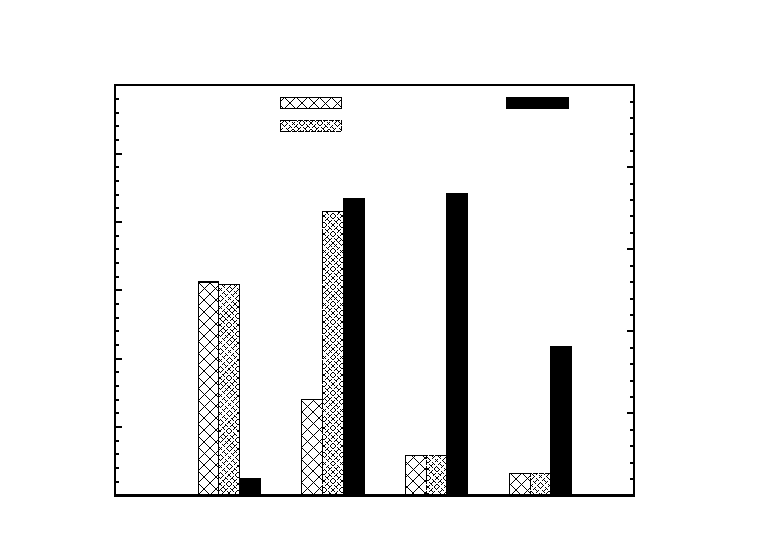
\includegraphics{conclusions-cs-en}}%
    \gplfronttext
  \end{picture}%
\endgroup

  \caption{
    Summary of the runtime benchmarking figures for the most relevant experiments
    with the Czech-English dataset (from left to right): baseline with the default
    parameters, baseline using multiple cores and large memory buffer, \eppex{}
    with no pruning and the \eppex{} with pruning configuration that achieved the best
    BLEU score of all experiments (labeled \emph{eppex defensive}).
  }
  \label{fig:conclusions-cs-en}
\end{figure}

\section{Future work}

We are aware, that in its current state, \eppex{} is a usable tool,
but a potential user of \eppex{} could be discouraged by the lack of some
finer control over its memory demands incurred during
runtime.

%\footnote{Without neglecting the importance of good program design,
%we cannot disregard the empirically determined principle that often the easiest
%and also cheapest solution to the performance limitations imposed by hardware
%is to buy better hardware. After all, no certain amount of memory is enough
%for all time.}

Addressing this possible concern, we see two possible ways to improve \eppex{}:
\begin{enumerate}
  \item Provide the user with a method to properly determine the maximum amount
    of memory that \eppex{} would require to process a particular training data.
  \item Provide the user with an option to set a limit on the maximum amount
    of memory utilized by the program.
\end{enumerate}

% VM peak estimation
In \Sref{sec:eppex-memory-demands} we already sketched a possible approach of how to determine
the memory peak of epochal extraction with a given pruning configuration and given input data.
However, it is hard to know whether this approach could be enhanced to offer
a more precise estimation than the 20\% overestimate based on the 25\% of training
data that we achieved in our initial experiments, and how consistent this estimation
could be made.

% Iterative deepening.
Point two has two possible approaches.
The first approach is to make the program aware of its memory consumption and implement
some means of resolving the situation when all available memory is exhausted.
The second approach is to control program memory consumption from outside:
as soon as its memory consumption exceeds a predefined limit, it can simply be terminated, 
and run again with harsher pruning (e.g. by raising the positive limit).
Obviously, the second approach does not require any changes to the existing version of
program, just a bit of scripting.

% Incremental training.
Besides finer control over memory consumption, yet another problem that could
be addressed in future work on \eppex{}, is the support for \emph{incremental
training}.
With new parallel data becoming available every year, more and more researchers seek
the means to retrain their translation models without running the whole
training process from scratch.

In a way, \eppex{} already helps work around this problem: by making the training
process much faster, the need to avoid rerunning the training process is somewhat
lowered.
However, a more straight-forward solution should be also possible.
Given that phrase tables usually contain the frequency counts of phrase pairs,
these frequencies could be used to initialize the internal Lossy Counting data
memory and the epochal extraction could then proceed by processing only the new
training data.


%%% Seznam použité literatury
\bibliographystyle{plainnat}
\bibliography{biblio}
\addcontentsline{toc}{chapter}{Bibliography}

%%% Tabulky v diplomové práci, existují-li.
%\chapwithtoc{List of tables}

%%% Použité zkratky v diplomové práci, existují-li, včetně jejich vysvětlení.
%\chapwithtoc{Seznam použitých zkratek}

%%% Přílohy k diplomové práci, existují-li (různé dodatky jako výpisy programů,
%%% diagramy apod.). Každá příloha musí být alespoň jednou odkazována z vlastního
%%% textu práce. Přílohy se číslují.
\appendix
\chapter{Installation}
\label{chap:installation}

% TODO: Pull-in eppex to the upstream Moses repository?
% \emph{Eppex} is shipped along with the Moses system and can be obtained the
% same way: by checking out Moses repository at Github.

\section*{Prerequisities}

Only Boost is required to compile and run \eppex{}.
If you had successfully compiled Moses then you probably already have all you need in place.

Just in case you did not want to install Boost as a whole, but only the necessary
parts of it, you will need to get two libraries (build them or install
them via your packaging system): \emph{Program Options} and \emph{IOStreams}.
\Eppex{} also requires working include path access to following
header-only libraries: \emph{Integer}, \emph{Iterator}, \emph{Pool} and \emph{Tokenizer}.

Besides that you will probably like to employ the power of hash tables
that comes with the recent version of C++ standard.\footurl{http://en.cppreference.com/w/cpp/container/unordered_set}
Most of decent C++ compilers will have this feature available,
although some may require to explicitly request compilation with C++11
features.\footnote{For example GCC requires the command-line parameter
\texttt{-std=c++0x} to be passed when compiling (or \texttt{-std=c++11}
with GCC 4.7 and later).}

\section*{Download}

\emph{Eppex} is hosted on Github\footurl{https://www.github.com} in
a fork\footurl{https://github.com/chesio/mosesdecoder}
of core Moses repository\footurl{https://github.com/moses-smt/mosesdecoder}.
If you have your own local clone of Moses repo then all you need is to add
the fork as a new remote, fetch from it and checkout the remote branch
\texttt{eppex} into some new local branch.
\begin{verbatim}
 cd <your-mosesdecoder-dir>
 git remote add eppex https://github.com/chesio/mosesdecoder.git
 git fetch eppex
 git checkout -b eppex eppex/eppex
\end{verbatim}

Important note: \eppex{} branch is based on \emph{RELEASE-1.0},
not the current master. Should you like to use \eppex{} with the most
recent Moses code, you may try merging branch \texttt{master} into \texttt{eppex}:
\begin{verbatim}
 git merge master
\end{verbatim}

Be warned that you may encounter some merge conflicts in \emph{train-model.perl}
as this script gets frequently updated.
In such a case feel free to contact the author of \eppex{},
he will be happy to help you.

\section*{Installation}

\Eppex{} related files may be found in \texttt{contrib/eppex} directory of \eppex{} fork
and for the time being the executable has to be compiled separately from the Moses
build.\footnote{For the build instructions on Moses consult the file \texttt{BUILD-INSTRUCTIONS.txt}.}
Some implementation features and functionality of \eppex{} is determined during compile-time
and you are encouraged to alter the defaults to suit your needs and your compiler capabilities.
The specific way of how to alter them depends on selected compilation method (\emph{Boost.Build} or
\emph{make} -- see below), the default behavior when no changes are made is following:
\begin{itemize}
  \item \eppex{} uses \verb|std::map| and \verb|std::set| as associative containers
  \item \eppex{} allows to extract phrase pairs of maximum length limit up to 8
\end{itemize}

Once compiled you will find \eppex{} binary in the \texttt{contrib/eppex} directory.
You are free to move it to whatever location suits your working environment,
just do not forget to pass the full path to \emph{train-model.perl} invocation.

\subsection*{Installation using Boost.Build}

This approach is recommended since \emph{Boost.Build}\footurl{http://www.boost.org/boost-build2/doc/html/index.html}
is required by Moses install process as well and if you do not have a working
\emph{Boost.Build} setup on your machine, you may try to use the one shipped with Moses:
just run \emph{bjam} shell script from Moses root instead of the system \emph{bjam}.\footnote{Note
that the first invocation will attempt to compile the actual \emph{bjam} executable from sources.}

If you would like to compile \eppex{} with faster (unordered) associative containers
just pass \texttt{--with-hashtables} flag to \emph{bjam} command.
The limit for maximum phrase length can be risen to 128 by adding
\texttt{--allow-long-phrases}.
\begin{verbatim}
  cd contrib/eppex
  bjam [--with-hashtables] [--allow-long-phrases]
  # or using Moses bjam: ../../bjam <options>
\end{verbatim}

\subsection*{Installation using make}
The \texttt{contrib/eppex} directory also contains a Makefile that may be used to compile
\eppex{} and should work on most Linux systems that have GCC compiler installed.
The faster associative containers and higher maximum phrase length limit can be activated
via environment variables:
\begin{verbatim}
  cd contrib/eppex
  [USE_HASHTABLES=1] [ALLOW_LONG_PHRASES=1] make all
\end{verbatim}

% In this chapter:
% - usage
% -- counting, extracting and scoring mode
% -- missing features

\chapter{Usage}
\label{chap:usage}

Depending on your goal, you may use \eppex{} to:
\begin{itemize}
 \item collect aggregated counts of phrase pairs of same lengths
 \item generate direct and inverse extract files -- acts as an alternative to \emph{extract} tool
 \item construct phrase table -- acts as an alternative to both \emph{extract} and \emph{score} tools
\end{itemize}

For any of the three options above, \eppex{} requires three input files to proceed:
the target side of corpus, the source side of corpus and the alignment information.
Moreover, if lexical scores are to be included in the phrase translation table,
both direct and inverse lexical translation tables have to be passed.

Eppex is a drop-in replacement, therefore it expects all input files to have the same
format as expected by \emph{extract} component and produces output files in the same
format as \emph{extract} and \emph{score} components.

\section{Lossy Counting parametrization}

For each phrase pair length (or an inclusive interval) a separate Lossy Counter
instance can be created that does its "lossy counting" separately from other instances
and is fed only with phrase pairs of length following into the assigned interval.
This allows to apply different limits (or thresholds) to phrase pairs of different length.
As quality benchmarking results presented in \Cref{chap:results} suggest, it is viable
to prune short phrase pairs with milder threshold (or no threshold at all) and use harsher
thresholds only for longer phrase pairs.

A \emph{phrase pair length} is defined as the length of its longest compound:
thus, a phrase pair $(e,f)$ with $e$ being "\emph{europe}" and $f$ being
"\emph{životě v evropě}" has the length of three.
This definition is motivated by the application of maximum phrase length limit
in core \emph{extract} tool: any phrase pair having either compound of length
exceeding the limit is not extracted (ie. the phrase length maximum is decisive).

\Eppex{} provides two ways to set \emph{support} and \emph{error} parameters
for Lossy Counting instances:
\begin{enumerate}
  \item You may specify the \emph{support} and \emph{error thresholds} directly, but doing so
    requires a good awareness of the amount of phrase pairs that is going to be fed into all
    instances of Lossy Counting algorithm, otherwise you can prune too much or do not prune at all.
  \item You may set the negative and positive limits that will directly relate to \emph{true}
    frequency counts of the phrase pairs extracted from your data. The \emph{negative limit}
    $n$ is such a value that no item whose true frequency is equal or less than $n$ will be output.
    The \emph{positive limit} $p$ is such a value that all items whose true frequency is equal
    or greater than $p$ will be output. Obviously, this forces $n < p$ (the only exception
    is the possibility to set $n = p = 0$).
\end{enumerate}

Within a single run of \eppex{} only one approach can be used.
The latter (limit-based) is much more convenient, thus recommended.
The only related draw-back is the necessity of reading the input files twice.
An additional loop over input files is done to grasp the counts of items
that will be fed to each Lossy Counter instance in order to calculate
the proper values of their \emph{support} and \emph{error} parameters,
so the properties of output will match the specified limits.\footnote{\Sref{sec:lossy-counting-definition}
provides more details on the relation between the positive and negative limits and
the support and error thresholds.}
However, this counting loop runs very fast and, as a matter of fact, all the \eppex{}
experiments reported in this work have been run in such a way and all the runtime
benchmarking statistics account for runs with this additional input processing loop.

\section{Command line options}

As already mentioned several times, \eppex{} is a command line tool.
The command line syntax for \emph{eppex} is following:\footnote{The order
of input files specification (first the target side, second the source side, third the alignment)
is the same as of \emph{extract} tool.}

\begin{verbatim}
  ./eppex tgt src align [dir-lex-table [inv-lex-table]] <options>
\end{verbatim}

The 5 positional arguments are:
\begin{itemize}
 \item \verb|tgt| - path to target language corpus (required).
  May be also provided via \verb|--tgt| option.
 \item \verb|src| - path to source language corpus (required).
  May be also provided via \verb|--src| option.
 \item \verb|align| - path to alignments file (required).
  May be also provided via \verb|--align| option.
 \item \verb|dir-lex-table| - path to direct lexical table (optional).
  May be also provided via \verb|--direct-lex-table| option. 
 \item \verb|inv-lex-table| - path to inverse lexical table (optional).
  May be also provided via \verb|--inverse-lex-table| option. 
\end{itemize}

Options related to phrase pairs counting:
\begin{itemize}
 \item \verb|--counts-file <string>| - path to file with phrase pairs counts.
  Turns on counting mode, if \verb|--reuse-counts| is not specified.
 \item \verb|--reuse-counts| - use counts from the provided file instead
  of counting anew (turns off counting mode).
 \item \verb|--max-phrase-len <num>| - maximum length of extracted phrases.
  Default value is 7. If one or more phrase length values or intervals
  are set via \verb|--limits| or \verb|--thresholds|, the maximum phrase
  length is set accordingly and any value provided via this option is ignored.
\end{itemize}

Options related to phrase pairs extraction:
\begin{itemize}
 \item \verb|--extract-file <string>| - path to file for extracted phrase pairs.
  The inverse file has \texttt{.inv} extension attached to its name automatically.
  Turns on extraction mode.
 \item \verb|--thresholds <string>| - a comma separated list of \emph{error} and \emph{support}
  thresholds for Lossy Counting. For each phrase pair length or range of lengths
  a separate lossy counter can be specified as a triple consisting of length/range
  specification, \emph{error} threshold and \emph{support} threshold joined with
  a colon sign, for example: \texttt{1:1e-10:1e-9} or \texttt{2-3:2e-7:3e-8}.
 \item \verb|--limits <string>| - a comma separated list of \emph{negative} and \emph{positive}
  limits for Lossy Counting. For each phrase pair length or range of lengths
  a separate lossy counter can be specified as a triple consisting of length or range
  specification, \emph{negative} limit and \emph{positive} limit joined with
  a colon sign, for example: \texttt{1-3:0:1} or \texttt{4:1:3}.
 \item \verb|--lambda <float>| - a value for parameter $\lambda \in (0.0, 1.0)$
  used in evaluation of the \emph{error} threshold $\epsilon$ from
  the positive limit $p$ and the negative limit $n$ as $\epsilon = (p - n - \lambda) / N$.
  Default value for $\lambda$ is 0.5.
 \item \verb|--no-final-pruning| - do not prune items with $f < (s - \epsilon)N$
  at the end of input processing, dump out all items remaining in storage.
\end{itemize}

Options related to phrase pairs scoring:
\begin{itemize}
 \item \verb|--phrase-table-file <string>| - path to phrase table file.
  Turns on scoring mode.
 \item \verb|--direct-lex-table <string>| - path to direct lexical table.
  If given, direct lexical score $lex(e|f)$ will be included in phrase table.
  May be passed also as 4-th positional parameter.
 \item \verb|--inverse-lex-table <string>| - path to inverse lexical table.
  If given, inverse lexical score $lex(f|e)$ will be included in phrase table.
  May be passed also as 5-th positional parameter.
 \item \verb|--OnlyDirect| - print only direct scores $p(e|f)$ and $lex(e|f)$
 \item \verb|--NoLex| - do not include lexical scores.
  It is sufficient to omit specification of lexical table files to not
  include lexical scores, but this switch can be used to override their presence.
 \item \verb|--NoPhraseCount| - do not include phrase counts.  
 \item \verb|--NoWordAlignment| - do not print word alignment.
 \item \verb|--GoodTuring| - adjust phrase translation probabilities with
  Good-Turing discounting
 \item \verb|--KneserNey| - adjust phrase translation probabilities with
  Kneser-Ney discounting
 \item \verb|--LogProb| - print logarithm of probabilities
 \item \verb|--NegLogProb| - print negative logarithm of probabilities
\end{itemize}

Options related to both phrase pairs extraction and scoring:
\begin{itemize}
 \item \verb|--GZOutput| - gzip the output (automatically
  adds \texttt{.gz} extension to the filenames provided).
\end{itemize}

It is important to mention that at least one of the options providing an output
file has to be set (\verb|--counts-file|, \verb|--extract-file| or \verb|--phrase-table-file|),
otherwise \eppex{} will be unable to decide on how to proceed.

Finally, three program options exist that provides some information about the program:
\begin{itemize}
 \item \verb|--help| - prints the program help.
 \item \verb|--info| - prints basic information about the program.
 \item \verb|--version| - prints program version.
\end{itemize}

\section{Missing features}

In the moment \eppex{} cannot extract orientation info data required for training
of reordering models.

Also some of the features of the core \emph{phrase-extract} suite from Moses
release 1.0 are yet missing in \eppex{}, namely:
\begin{itemize}
  \item inclusion of sentence ID in extract files: see \verb|--IncludeSentenceId|
    option of \emph{extract} tool
  \item adding sentence weights to extracted phrases: see \verb|--InstanceWeights|
    option of \emph{extract} tool
  \item dumping singleton feature: see \verb|--Singleton| option of \emph{scorer} tool
  \item adding penalty to unaligned (function) words: see \verb|--UnalignedPenalty|
    and \verb|--UnalignedFunctionWordPenalty| options of \emph{scorer} tool
\end{itemize}

\section{Examples}

Let us finish this chapter with some examples that demonstrate some typical
patterns of \eppex{} usage. Because input files specification is always required,
we will only mark it by \verb|<input>| in command line snippets below.

Grab counts of phrase pairs of lengths up to 8 that would be extracted from
input corpus and store them in the file \texttt{counts.txt}:
\begin{verbatim}
  eppex <input> --max-phrase-len 8 --counts-file counts.txt
\end{verbatim}

Construct phrase table reusing the counts from file \texttt{counts.txt} and using
two Lossy Counting instances: one to keep all phrase pairs with length from
1 to 3 and another to remove all phrase pairs with length from 4 to 6 with true
frequency equal to 1 and keep all with true frequency at least 3. Despite the
\texttt{counts.txt} file contains counts for phrase pairs lengths up to 8,
the specification of \verb|--limits| determines that phrase table will contain
only phrase pairs of length up to 6:
\begin{verbatim}
  eppex <input> --counts-file counts.txt --reuse-counts \\
    --limits 1-3:0:1,4-6:1:3 --phrase-table-file phrase-table
\end{verbatim}

Construct phrase table with phrase pairs pruned according to the following rule:
for each phrase pair length $L$ only phrase pairs with true frequency at least
$L$ will be retained, the rest might or might not be pruned depending on the
distribution of their occurrences in parallel corpus:
\begin{verbatim}
  eppex <input> --phrase-table-file phrase-table \\
    --limits 1:0:1,2:0:2,3:0:3,4:0:4,5:0:5,6:0:6,7:0:7
\end{verbatim}

Construct complete phrase table not removing a single phrase pair.
The phrase table will be stored gzipped in file \texttt{phrase-table.gz}
and will contain phrase pairs of length up to (default maximum) 7.
\begin{verbatim}
  eppex <input> --phrase-table-file phrase-table --GZOutput
\end{verbatim}


\openright
\end{document}
